\documentclass[11pt,twoside,openright,italian]{book} %Use "italian" to show bibliography enties in italian and "english" to show them in english
\usepackage[utf8]{inputenc}
\usepackage{subcaption}
\usepackage{babel}
\usepackage{csquotes}
\usepackage{multirow}

\usepackage{listings}
\usepackage{color}
\definecolor{lightgray}{rgb}{.9,.9,.9}
\definecolor{darkgray}{rgb}{.4,.4,.4}
\definecolor{purple}{rgb}{0.65, 0.12, 0.82}

\lstdefinelanguage{JavaScript}{
  keywords={typeof, new, true, false, catch, function, return, null, catch, switch, var, let, if, in, while, do, else, case, break, continue},
  keywordstyle=\color{blue}\bfseries,
  ndkeywords={class, export, boolean, throw, implements, import, this},
  ndkeywordstyle=\color{darkgray}\bfseries,
  identifierstyle=\color{black},
  sensitive=false,
  comment=[l]{//},
  morecomment=[s]{/*}{*/},
  commentstyle=\color{purple}\ttfamily,
  stringstyle=\color{red}\ttfamily,
  morestring=[b]',
  morestring=[b]"
}

\lstdefinelanguage{Bash}{
  keywords={cd, ls, ls -l, rm, sudo, install, run, add, serve, build},
  keywordstyle=\color{blue}\bfseries,
  ndkeywords={},
  keywordstyle=\color{blue}\bfseries,
  ndkeywordstyle=\color{darkgray}\bfseries,
  identifierstyle=\color{black},
  sensitive=false,
  comment=[l]{//},
  morecomment=[s]{/*}{*/},
  commentstyle=\color{purple}\ttfamily,
  morestring=[b]',
  morestring=[b]"
}

\lstset{
   language=JavaScript,
   backgroundcolor=\color{lightgray},
   extendedchars=true,
   basicstyle=\footnotesize\ttfamily,
   showstringspaces=false,
   showspaces=false,
   numbers=left,
   numberstyle=\footnotesize,
   numbersep=9pt,
   tabsize=2,
   breaklines=true,
   showtabs=false,
   captionpos=b
}

\interfootnotelinepenalty=10000 %Prevents footnotes splitting across pages
\usepackage{siunitx}
\sisetup{%
  inter-unit-product=\ensuremath{{}\cdot{}},
  per-mode=symbol
  }
\usepackage{newtxtext,newtxmath,amsmath}
\usepackage{float}
\usepackage{ifthen}

\newcommand{\nomunit}[1]{\renewcommand{\nomentryend}{\hspace*{\fill}[#1]}}

\newcounter{savepage}
\usepackage[dvipsnames]{xcolor}
\usepackage{wallpaper}
%\usepackage[acronym,toc,shortcuts,translate=babel,nopostdot]{glossaries}
%\usepackage{glossary-mcols} % glossary in columns
\usepackage{float}
%\makeglossaries
%\glstoctrue
\usepackage{float}
\setcounter{secnumdepth}{4}
\setcounter{tocdepth}{4}
\usepackage{indentfirst}
\renewcommand{\baselinestretch}{1.3}
\usepackage{graphicx}
\graphicspath{ {Immagini/} }
\usepackage{caption}
\usepackage[a4paper,
			nomarginpar,
            left=30mm,
            right=30mm,
            top=40mm,
            bottom=40mm]{geometry}
\usepackage{lipsum}
\usepackage{enumitem}

\usepackage{listings}
\usepackage{xcolor}
 
\definecolor{codegreen}{rgb}{0,0.6,0}
\definecolor{codegray}{rgb}{0.5,0.5,0.5}
\definecolor{codepurple}{rgb}{0.58,0,0.82}
\definecolor{backcolour}{rgb}{0.95,0.95,0.92}
 
\lstdefinestyle{mystyle}
{
    backgroundcolor=\color{backcolour},   
    commentstyle=\color{codegreen},
    keywordstyle=\color{magenta},
    numberstyle=\tiny\color{codegray},
    stringstyle=\color{codepurple},
    basicstyle=\ttfamily\footnotesize,
    breakatwhitespace=false,         
    breaklines=true,                 
    captionpos=b,                    
    keepspaces=true,                 
    numbers=left,                    
    numbersep=5pt,                  
    showspaces=false,                
    showstringspaces=false,
    showtabs=false,                  
    tabsize=2
}

\lstset{style=mystyle}

\setlist[enumerate]{itemsep=-1mm}
\marginparpush=0pt

\usepackage{fancyhdr}
\pagestyle{fancy}
\setlength{\headheight}{26pt}
\renewcommand{\chaptermark}[1]{\markboth{#1}{}}
\renewcommand{\sectionmark}[1]{\markright{#1}}
\fancyhf{}
\fancyhead{}
\fancyhead[C]{\hyperref[Indice_generale]{Indice} > \hyperlink{part::\theHpart}{Parte \theHpart} > \hyperlink{chapter::\theHchapter}{\theHchapter\ \leftmark} > \hyperlink{section::\theHsection}{\theHsection\ \rightmark}}
\fancyfoot{}
\fancyfoot[C]{\thepage}

\newcommand\blfootnote[1]{% %footnote without number: \blfootnote{examole}
  \begingroup
  \renewcommand\thefootnote{}\footnote{#1}%
  \addtocounter{footnote}{-1}%
  \endgroup
}

\usepackage{mathtools}
\newtagform{equationwithname}{Equazione }{}

\renewcommand{\headrulewidth}{0.4pt}
\renewcommand{\footrulewidth}{0.4pt}
\renewcommand{\chaptername}{Capitolo}
\renewcommand{\appendixname}{Appendice}
\renewcommand{\listfigurename}{Indice delle figure}
\renewcommand{\contentsname}{Indice generale}
\renewcommand{\listtablename}{Indice delle tabelle}
\renewcommand{\figurename}{Fig.}
\renewcommand{\tablename}{Tabella}
\renewcommand{\partname}{Parte}
\usepackage[backend=biber,
            citestyle=verbose-ibid,
            sorting=none,
%            citereset=part, % Not working, using chngcntr and counterwithout
            bibstyle=numeric,
            autocite=footnote,
            doi=true,
            url=true,
            maxnames=99, % Show all authors in citation footnotes and bibliography
            ]{biblatex}

\defbibenvironment{bibliography} % Enumeration of entries in bibliography
  {\enumerate
     {}
     {\setlength{\leftmargin}{\bibhang}%
      \setlength{\itemindent}{-\leftmargin}%
      \setlength{\itemsep}{\bibitemsep}%
      \setlength{\parsep}{\bibparsep}}}
  {\endenumerate}
  {\item}

\makeatletter

\renewbibmacro*{cite:full}{
  \usebibmacro{cite:full:citepages}
  \printtext[bibhypertarget]{
    \usedriver
      {\DeclareNameAlias{sortname}{default}}
      {\thefield{entrytype}}}
  \usebibmacro{shorthandintro}
  \csxdef{cbx@\thefield{entrykey}@footnotenumber}{\the\value{footnote}}
}

\DeclareFieldFormat{prefixnumber}{}
\DeclareFieldFormat{labelnumber}{\csuse{cbx@\thefield{entrykey}@footnotenumber}}

\makeatother

\usepackage{chngcntr}
\counterwithout*{footnote}{chapter}
\renewcommand*\thefootnote{\textcolor{Sepia}{[\arabic{footnote}]}}
\addbibresource{Testo/Z04_Bibliografia.bib}
\setlength\bibitemsep{3.0\itemsep}
\usepackage{adjustbox}
%\usepackage{showframe}
\usepackage[bookmarks]{hyperref}
\usepackage[open,openlevel=0]{bookmark}
\usepackage{hyperref}
\hypersetup{colorlinks=true,
            urlcolor=blue,
            linkcolor=MidnightBlue,
            citecolor=red,
            bookmarksopen=true,
            pdfstartview={Fit},
            pdffitwindow=true,
			breaklinks=true,
            pdftitle={Documentazione del lavoro di gruppo - Informatica III - Modulo Progettazione e Algoritmi (Cognome-A, Cognome-B, Cognome-C)},
			pdfauthor={Nome-A Cognome-A, Nome-B Cognome-B, Nome-C Cognome-C},
            pdfsubject={Documentazione per il lavoro di gruppo - Informatica III - Modulo Progettazione e Algoritmi},
            pdfcreator={Nome-A Cognome-A, Nome-B Cognome-B, Nome-C Cognome-C},
            pdfproducer={Nome-A Cognome-A, Nome-B Cognome-B, Nome-C Cognome-C},
            pdfkeywords={documentazione, lavoro di gruppo, informatica III, Modulo Progettazione e Algoritmi, software, programma, sito web, website, documentation, group work, software design, software engineering, computer engineering, computer science, Scandurra, Patrizia Scandurra},
            }
\title{Documentazione del lavoro di gruppo - Informatica III - Modulo Progettazione e Algoritmi}
\author{Nome-A Cognome-A, Nome-B Cognome-B, Nome-C Cognome-C}
\date{24 January 2020}

\begin{document}
\usetagform{equationwithname}
\frontmatter
\begin{titlepage}
    \begin{center}
        
\includegraphics[scale=0.5]{Immagini/logo.png}
        \Huge{\textbf{Documentazione di progetto}}\\
        \huge{Lavoro di gruppo - Corso di Informatica III - Modulo Progettazione e Algoritmi}
        
        \vspace{0.5cm}
        \normalsize
        \begin{tabular}{rl}
        \centering
            \begin{tabular}{rr}
                \textbf{Studenti:} & \\
                \\
                \\
                {Docente:} & \\
            \end{tabular} &
            \begin{tabular}{l}
                \textbf{Nome-A Cognome-A, Matr. 0000000}\\
                \textbf{Nome-B Cognome-B, Matr. 0000000}\\
                \textbf{Nome-C Cognome-C, Matr. 0000000}\\
                Prof.ssa Patrizia Scandurra\\
            \end{tabular}\\
            & \\
            \begin{tabular}{r}
            {
                \label{fig:Logo UniBG}}
            \end{tabular} &
            \begin{tabular}{l}
                CdL Magistrale in Ing. Informatica\\
                Facoltà di Ingegneria\\
                Università degli Studi di Bergamo\\
            \end{tabular}\\
            & \\
            \begin{tabular}{l}
            \end{tabular} &
            \begin{tabular}{l}
            Bergamo, Italia - Gennaio 2020\\
            \end{tabular}\\
        \end{tabular}\\
    \end{center}
\end{titlepage} \label{Copertina}
\bookmark[dest=Cover]{Copertina}

\newpage\null\thispagestyle{empty}\newpage

{\pagestyle{plain}
\tableofcontents
\cleardoublepage}
\addcontentsline{toc}{chapter}{Indice generale} \label{Indice_generale}

{\pagestyle{plain}
\listoffigures
\addcontentsline{toc}{chapter}{Indice delle figure} \label{Indice_delle_figure}
\cleardoublepage}

\listoftables
\addcontentsline{toc}{chapter}{Indice delle tabelle} \label{Indice_delle_tabelle}

\setcounter{savepage}{\arabic{page}}

%\newpage\null\thispagestyle{empty}\newpage

\mainmatter
\setcounter{page}{\thesavepage+2}

\setcounter{part}{-1}
\part{Iterazione 0} \hypertarget{part::\theHpart}{}

\setcounter{chapter}{0}

\chapter{Introduzione} \label{chap:Introduzione} \hypertarget{chapter::\theHchapter}{}
\section{Panoramica} \hypertarget{section::\theHsection}
Il problema del riscaldamento climatico globale e dei disastri ambientali degli ultimi anni, ha portato alla crescente rigidezza delle normative sulle emissioni e quindi ad un aumento di volume del mercato delle auto elettriche e ibride a scapito di quelle termiche.

Insieme all'arrivo dei veicoli elettrificati sono sorti anche i problemi della ricarica di tali veicoli dovuti alla scarsa estensione della rete di colonnine atte a tale scopo.

L'obiettivo del nostro progetto è quello di creare una Web App che semplifichi gli spostamenti agli utilizzatori di veicoli elettrici, consentendo loro di pianificare itinerari tenendo in considerazione anche l'esigenza di ricarica.

\chapter{Analisi dei requisiti} \label{chap:Analisi dei requisiti} \hypertarget{chapter::\theHchapter}{}
\section{Analisi del contesto} 
\hypertarget{section::\theHsection}
Allo stato attuale l'unico Software in grado di creare un planner per veicoli elettrici è quello installato nei veicoli Tesla, la nota casa automobilistica americana, leader in questo settore. Questo Software inoltre si integra con la vettura e consente di monitorarne lo stato e controllarla da remoto.

Purtroppo però il suo utilizzo è riservato ai soli possessori di un'auto dello stesso marchio; rimangono quindi scoperti tutti coloro che hanno acquistato un veicolo elettrico di un diverso produttore. Per loro l'unica applicazione disponibile è quella reperibile al link \url{http://evroute.controtex.com} che, però, fa riferimento solo al territorio inglese. Non è quindi disponibile alcun servizio relativo al suolo italiano. 

\section{Studio di fattibilità}
\hypertarget{section::\theHsection}
Per realizzare le funzionalità che abbiamo ideato avremo bisogno di 4 elementi: una mappa, un pianificatore del percorso iniziale, un database delle stazioni di ricarica e infine una componente che si occupi di unire il percorso fornito con la posizione delle colonnine per generare il percorso con le eventuali fermate.

\chapter{Usecases} \label{chap:Usecases} \hypertarget{chapter::\theHchapter}{}
\section{Descrizione delle usecases} \hypertarget{section::\theHsection}
In questa sezione andremo a schematizzare i requisiti funzionali del software da sviluppare, essi sono indipendenti dalla tipologia di tecnologia utilizzata, dall'architettura, dalla piattaforma e dalla tipo di linguaggio di programmazione scelto.

Nel nostro caso avremo un attore Utente che interagisce con il sistema, questi potrà invocare una Richiesta Percorso(UC1) che a sua volta include un altro caso d'uso che si occuperà della generazione del percorso(UC2).

Generazione percorso fa utilizzo di due API esterne: Open Street Map si occuperà di fornire una mappa del percorso (planner) mentre Open Charge Map è un database contente tutte le informazioni sulla posizione delle colonnine di ricarica.

L'Utente potrà Registrarsi(UC8) ed effettuare un Login(UC10) all'applicazione web in modo da ottenere dei Servizi Aggiuntivi(UC3).

I servizi aggiuntivi offerti sono il Salvataggio dei Luoghi Preferiti(UC4), Modifica Dati Utente(UC5), Esportare il Percorso(UC6), Generazione dei Report(UC7), Cancellazione Utente(UC9) e il Logout(UC11).
\\\\\\\\\\\\\\\\

\begin{figure}[htp]
\centering
{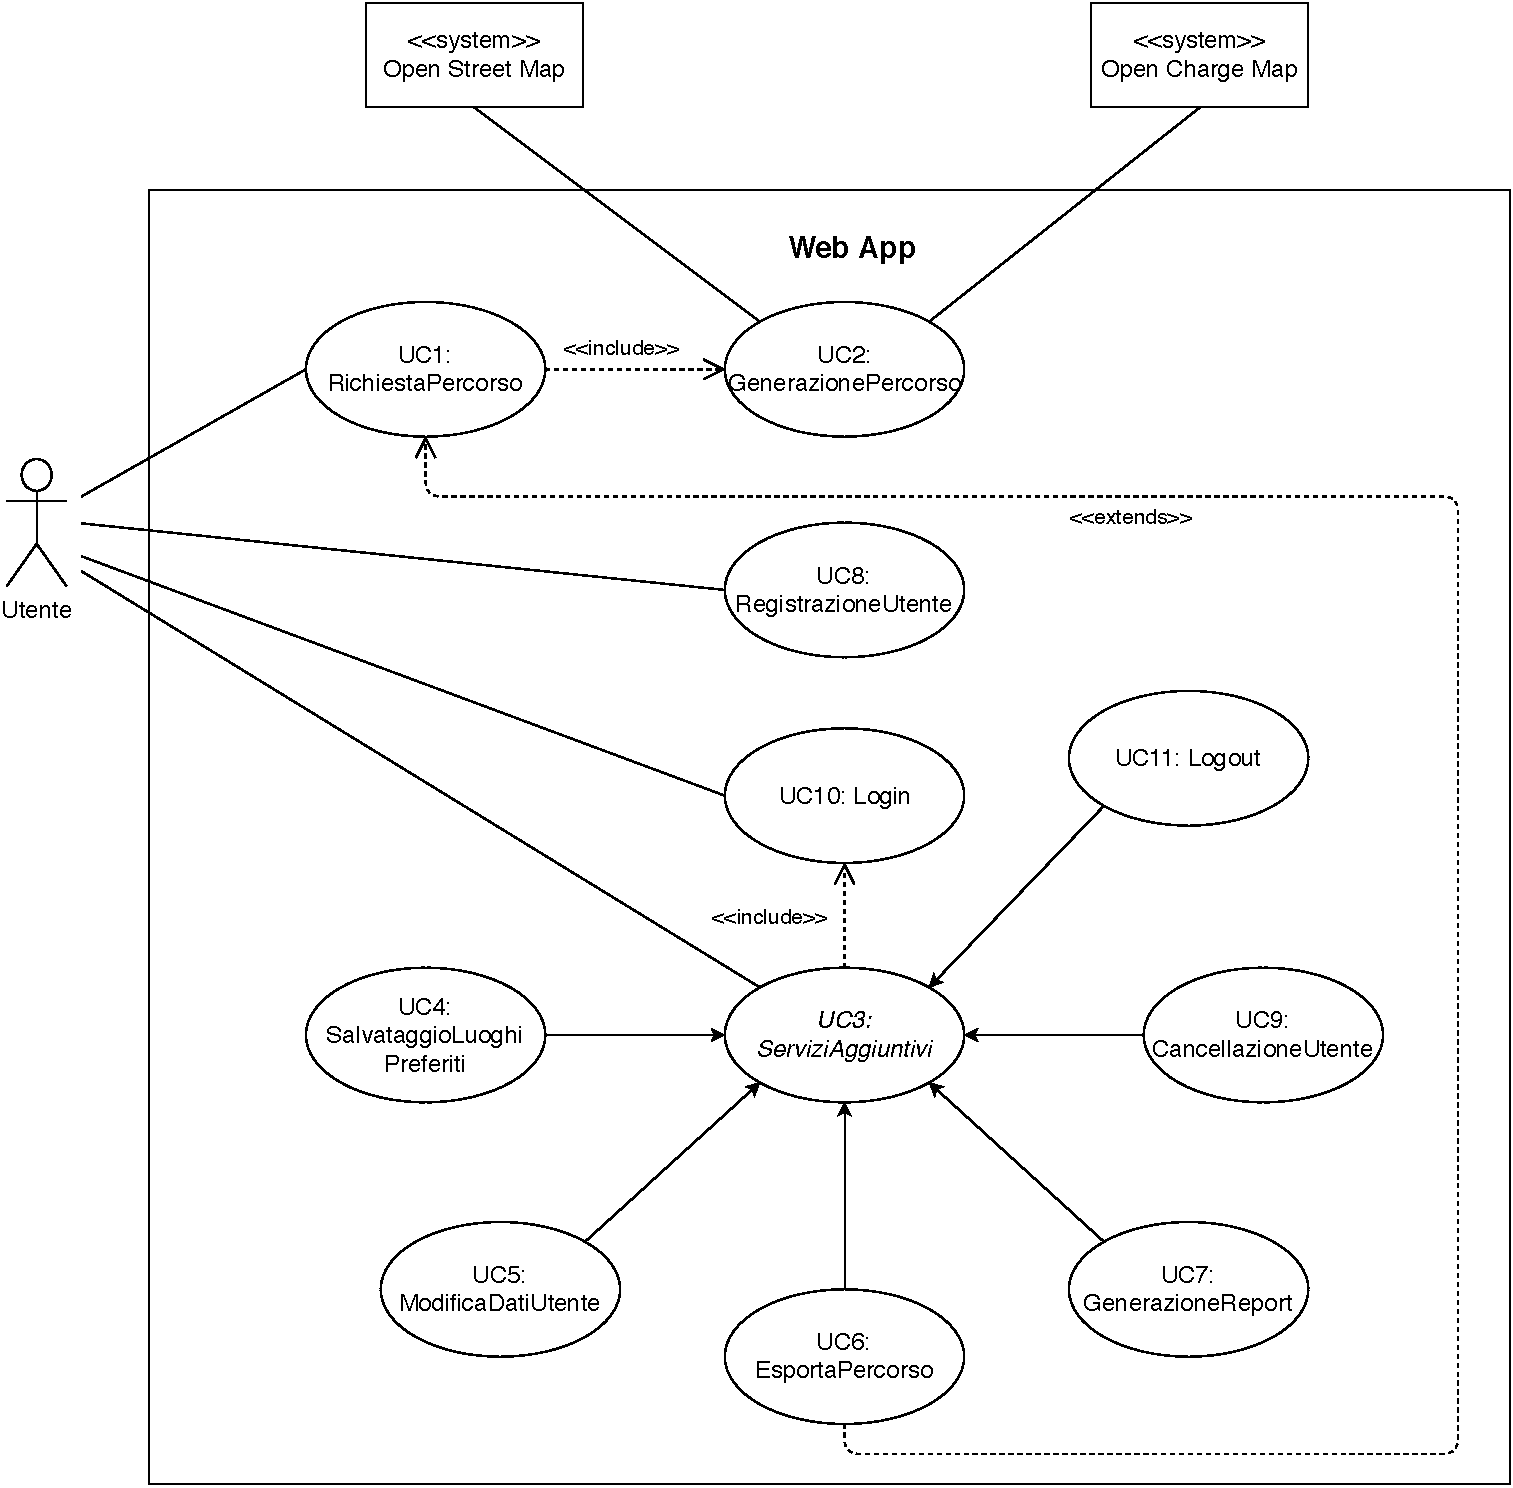
\includegraphics[scale=0.55]{Immagini/UseCases.pdf}}
\caption{Diagramma dei casi d'uso\label{t1v2}}
\end{figure}

\underline{\textbf{UC1: RichiestaPercorso}}

\begin{enumerate}
\item\textbf{Descrizione} \\ L'utente desidera ottenere il tragitto fra due località comprensivo delle soste da effettuare presso le colonnine di ricarica. %Vuole inoltre conoscere la durata della sosta presso ogni colonnina.
\item\textbf{Requisiti coperti}\\ /
\item\textbf{Attori} \\ Utente
\item\textbf{Precondizioni} \\ L'utente ha accesso alla pagina web ed è pronto ad inserire i dati richiesti
\item\textbf{Passi principali}
\begin{enumerate}
\item L'utente inserisce la località di partenza, quella di destinazione desiderata e l'autonomia dell'auto
\item Controllo che le località di inizio, fine percorso e autonomia sono inserite con la giusta formattazione 
\item Controllo che le località inserite sono valide e che l'autonomia sia stata inserita correttamente(valori negativi non ammessi)
\item Le informazioni circa le località inserite dall'utente vengono processate attraverso Open Street Map al fine di convertire gli indirizzi in coordinate
\item Le coordinate vengono inviate al modulo di analisi con il relativo campo autonomia
\end{enumerate}
\item\textbf{Situazioni eccezionali} \\ /
\item\textbf{Postcondizioni} \\ Coordinate formattate
\end{enumerate}

\underline{\textbf{UC2: GenerazionePercorso}}

\begin{enumerate}
\item\textbf{Descrizione} \\ Generazione del percorso finale comprensivo di soste per le ricariche dell'auto
\item\textbf{Requisiti coperti} \\ R1
\item\textbf{Attori} \\ /
\item\textbf{Precondizioni} \\ Coordinate formattate
\item\textbf{Passi principali}
    \begin{enumerate}
    \item Le coordinate ricevute vengono fornite a Open Street Map per ottenere il percorso fra i due punti
    \item Il percorso ottenuto viene combinato con i dati delle colonnine per generare il percorso definitivo
    \item Il risultato viene presentato all'utente sia in forma grafica che testuale
    \end{enumerate}
\item\textbf{Situazioni eccezionali} \\ Non esiste un percorso stradale fra le due località
\item\textbf{Postcondizioni} \\ Percorso generato
\end{enumerate}

\underline{\textbf{UC3: ServiziAggiuntivi}}
\begin{enumerate}
\item\textbf{Descrizione}\\
Use Case astratto che rappresenta i servizi ulteriori a cui un utente registrato può accedere
\item\textbf{Requisiti coperti}\\ /
\item\textbf{Attori}\\ Utente
\item\textbf{Precondizioni}\\ Utente loggato
\item\textbf{Passi principali}\\ /
\item\textbf{Situazioni eccezionali}\\ /
\item\textbf{Postcondizioni}\\ /
\end{enumerate}

\underline{\textbf{UC4: SalvataggioLuoghiPreferiti}}

\begin{enumerate}
\item\textbf{Descrizione}\\
L'utente può salvare i suoi luoghi preferiti (i.e. i luoghi maggiormente visitati), in modo da potervi accedere più facilmente (non sarà necessario digitare ogni volta l'indirizzo completo)
\item\textbf{Requisiti coperti}\\ R7
\item\textbf{Attori}\\ Utente
\item\textbf{Precondizioni}\\ Utente loggato
\item\textbf{Passi principali}
\begin{enumerate}
    \item L'utente inserisce il luogo da salvare
    \item L'utente da un nome al luogo in questione (es. Casa, Lavoro, etc.)
    \item L'utente preme sul pulsante salva dati
    \item Il sistema risponde con un avvenuto salvataggio
\end{enumerate}
\item\textbf{Situazioni eccezionali}\\ Dati inseriti non validi
\item\textbf{Postcondizioni}\\ /
\end{enumerate}


\underline{\textbf{UC5: ModificaDatiUtente}}

\begin{enumerate}
\item\textbf{Descrizione}\\
L'utente può modificare i dati inseriti in fase di registrazione
\item\textbf{Requisiti coperti}\\
R3
\item\textbf{Attori}\\
Utente
\item\textbf{Precondizioni}\\ Utente loggato
\item\textbf{Passi principali}
\begin{enumerate}
    \item L'utente inserisce i dati da modificare nel sistema
    \item L'utente preme sul pulsante salva dati
    \item Il sistema risponde con un avvenuto salvataggio
\end{enumerate}
\item\textbf{Situazioni eccezionali}\\
Dati inseriti non validi
\item\textbf{Postcondizioni}\\
/
\end{enumerate}

\underline{\textbf{UC6: EsportaPercorso}}

\begin{enumerate}
\item\textbf{Descrizione}\\
L'utente può esportare il percorso generato dall'applicazione in diversi formati o può condividerlo su diverse piattaforme social
\item\textbf{Requisiti coperti}\\
R4
\item\textbf{Attori}\\
Utente
\item\textbf{Precondizioni}\\
Utente loggato, Percorso generato
\item\textbf{Passi principali}
\begin{enumerate}
    \item L'utente può esportare la pianificazione tramite un apposito pulsante "esporta" che fornisce diverse opzioni tramite un menù a comparsa
\end{enumerate}
\item\textbf{Situazioni eccezionali}\\ /
\item\textbf{Postcondizioni}\\ /
\end{enumerate}

\underline{\textbf{UC7: GenerazioneReport}}

\begin{enumerate}
\item\textbf{Descrizione}\\
L'utente può visualizzare alcune statistiche di suo interesse circa lo storico dei suoi viaggi (es. totale kilometri percorsi, strade maggiormente frequentate, tempo di sosta medio alle colonnine, frequenza media di sosta, etc.)
\item\textbf{Requisiti coperti}\\
R5
\item\textbf{Attori}\\
Utente
\item\textbf{Precondizioni}\\ Utente loggato
\item\textbf{Passi principali}\\ /
\item\textbf{Situazioni eccezionali}\\ /
\item\textbf{Postcondizioni}\\
/
\end{enumerate}

\underline{\textbf{UC8: RegistrazioneUtente}}
\begin{enumerate}
\item\textbf{Descrizione}\\
L'utente può registrarsi all'applicazione in modo da avere accesso ad ulteriori funzioni
\item\textbf{Requisiti coperti}\\
R2
\item\textbf{Attori}\\
Utente
\item\textbf{Precondizioni}\\ /
\item\textbf{Passi principali}
\begin{enumerate}
\item L'utente preme il pulsante di registrazione presente nell'interfaccia
\item L'utente inserisce i propri dati nella schermata di registrazione
\item L'utente preme sul pulsante invio dati al sistema
\item Il sistema risponde con un avvenuta registrazione e salva i dati dell'utente
\end{enumerate}
\item\textbf{Situazioni eccezionali}\\
Utente già registrato
\item\textbf{Postcondizioni}\\
Utente registrato 
\end{enumerate}

\underline{\textbf{UC9: CancellazioneUtente}}
\begin{enumerate}
\item\textbf{Descrizione}\\
L'utente può cancellare il suo account ed eliminare i suoi dati
\item\textbf{Requisiti coperti}\\
/
\item\textbf{Attori}\\
Utente
\item\textbf{Precondizioni}\\ Utente loggato
\item\textbf{Passi principali}
\begin{enumerate}
\item L'utente preme il pulsante di cancellazione account
\item Il server informa l'utente circa l'irreversibilità dell'operazione e la perdita dei dati
\item L'utente preme sul pulsante conferma
\item Il sistema richiede la password dell'utente
\item L'utente inserisce la password
\item Il server verifica la correttezza della password, elimina l'account e invia una conferma all'utente sul buon esito dell'operazione
\end{enumerate}
\item\textbf{Situazioni eccezionali}\\
Password fornita errata
\item\textbf{Postcondizioni}\\
Utente cancellato
\end{enumerate}

\underline{\textbf{UC10: Login}}
\begin{enumerate}
\item\textbf{Descrizione}\\
L'utente accede al sistema con le sue credenziali
\item\textbf{Requisiti coperti}\\ /
\item\textbf{Attori}\\
Utente
\item\textbf{Precondizioni}\\ Utente registrato
\item\textbf{Passi principali}
\begin{enumerate}
\item L'utente preme sul pulsante di login
\item L'utente inserisce i propri dati nella schermata 
\item L'utente preme sul pulsante invio dati al sistema
\item Il sistema risponde con una conferma
\end{enumerate}
\item\textbf{Situazioni eccezionali}\\
Dati forniti errati
\item\textbf{Postcondizioni}\\
Utente loggato
\end{enumerate}

\underline{\textbf{UC11: Logout}}
\begin{enumerate}
\item\textbf{Descrizione}\\
L'utente esce dal suo account
\item\textbf{Requisiti coperti}\\ /
\item\textbf{Attori}\\
Utente
\item\textbf{Precondizioni}\\ Utente loggato
\item\textbf{Passi principali}
\begin{enumerate}
\item L'utente preme sul pulsante di logout
\item Il sistema risponde con una conferma
\end{enumerate}
\item\textbf{Situazioni eccezionali}\\ /
\item\textbf{Postcondizioni}\\
Utente non loggato
\end{enumerate}



\section{Diagramma comportamentale} \hypertarget{section::\theHsection}
Il diagramma comportamentale descrive come evolve il software (Fig.3.2).

In particolare un utente interroga il server e questi risponde con il caricamento della pagina web richiesta (Web page loaded).
L'utente inserisce i dati richiesti nei campi e sottomette la richiesta al sistema(Request submitted).
Una volta calcolato il percorso migliore il sistema risponde a schermo con la visualizzazione della mappa.


\begin{figure}[htb]
\centering
{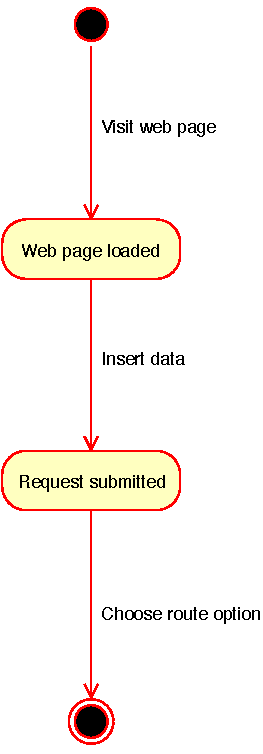
\includegraphics[scale=1]{Immagini/Automa_stati_finiti.pdf}}
\caption{Diagramma comportamentale}
\end{figure}


\chapter{Specifiche} \label{chap:Specifiche} \hypertarget{chapter::\theHchapter}{}
\section{Introduzione specifiche} \hypertarget{section::\theHsection}
In questo capitolo analizzeremo le specifiche funzionali e non funzionali della applicazione da sviluppare.

La priorità di una funzione è scelta in base a quante funzioni dipendono da essa:

\begin{enumerate}
\item \textbf{Alta}: è fondamentale implementarla prima di procedere con il macroblocco delle funzioni con
media priorità. Sono funzioni da implementare principalmente l’una in serie con l’altra.
\item \textbf{Media}: è fondamentale implementarla prima di procedere con il macroblocco delle funzioni
con bassa priorità. È possibile implementare parallelamente queste funzioni.
\item \textbf{Bassa priorità}: da loro non dipende nessuna funzione.
\end{enumerate}

\section{Specifiche funzionali} \hypertarget{section::\theHsection}
Le specifiche funzionali dell'applicazione sono le seguenti:
\begin{enumerate}
\item \textbf{Calcolo del percorso}: una volta fornito la mappa delle colonnine e il percorso da un punto A ad un punto B l'app deve rielaborare i dati in modo da calcolare il nuovo percorso comprensivo di eventuali soste.
\item \textbf{Iscrizione utente}: l'applicazione deve poter permettere all'utente l'iscrizione in modo da avere ulteriori servizi.
\item \textbf{Modifica dati utente}: l'applicazione deve poter permettere all'utente la modifica dei propri dati all'interno del proprio profilo.
\item \textbf{Esportazione tragitto}: quando l'applicazione restituisce un percorso all'utente, questi deve essere in grado di esportarlo in un formato opportuno.
\item \textbf{Visualizzazioni statistiche}: l'utente dal proprio profilo è in grado di visualizzare le statistiche relative ai propri viaggi.
\item \textbf{Mostra alternative percorso}: l'applicazione può mostrare all'utente le alternative al percorso precedentemente calcolato.
\item \textbf{Memorizzazione luoghi preferiti}: l'utente è in grado di salvare i percorsi preferiti nel proprio profilo
\item \textbf{Visualizzazione percorso}: l'utente è in grado di vedere il percorso calcolato dall'algoritmo su una mappa.
\item \textbf{Visualizza dati utente}: l'utente è in grado di vedere i propri dati nell'apposito profilo utente.
\end{enumerate}

Sono riportati in Tabella 4.1 tutte le specifiche funzionali con le relative priorità.

\begin{table}[h]
\centering
\begin{tabular}{|c|l|c|c|}
\hline
Codice & Nome                            & Priorità & Implementato \\ \hline
R1     & Calcolo percorso                & A        & SI           \\ \hline
R2     & Iscrizione utente               & M        & NO           \\ \hline
R3     & Modifica dati utente            & B        & NO           \\ \hline
R4     & Esportazione tragitto           & M        & NO           \\ \hline
R5     & Visualizzazione statistiche     & B        & NO           \\ \hline
R6     & Mostra alternative percorso     & A        & NO           \\ \hline
R7     & Memorizzazione luoghi preferiti & M        & NO           \\ \hline
R8     & Visualizza percorso             & A        & SI           \\ \hline
R9     & Visualizza dati utente          & M        & NO           \\ \hline
\end{tabular}
\caption{Specifiche funzionali, priorità e implementazione}
\end{table}

\chapter{Architettura} \label{chap:Architettura} \hypertarget{chapter::\theHchapter}{} \section{Deployment Diagram} \hypertarget{section::\theHsection}
Il deployment diagram mostrato nella Figura 5.1 del sistema evidenzia quali dispositivi vengono considerati, le interconnessioni tra loro e dove le componenti software verranno istanziate.

Nel nostro caso abbiamo 4 "device":\\
Un device è rappresentato dal Client che tramite protocollo http invia una richeista al device Server, esso al suo interno presenta una componente Web Browser che si interfaccerà con il Server.

Sono presenti due device di supporto alla nostra applicazione: Open Charge Map Server e Open Street Map Server queste due componenti restituiscono tramite una richiesta di tipo REST la posizione delle colonnine e il percorso da un punto di partenza ad un punto di destinazione richiesto dall'utente.
Il cuore del nostro software è presente dentro il device Server in cui sono presenti 5 componenti. Il componente charger\textunderscore location\textunderscore data\textunderscore feeder si occupa di scaricare le colonnine tramite l'API di Open Charge Map e le passa al modulo general\textunderscore data\textunderscore bank che contiene i metodi atti a generare la struttura dati che svolgerà il ruolo di database locale. itinerary\textunderscore feeder è il modulo che calcola il percorso attraverso l'API di Open Street Map. Il componente algorithm\textunderscore calculation incorpora l'algoritmo che si occuperà di trovare le colonnine a cui fermarsi. Infine client\textunderscore communication si occupa di ricevere gli input dall'utente e di restituire il risultato a schermo. 



\begin{figure}[htp]
\centering
{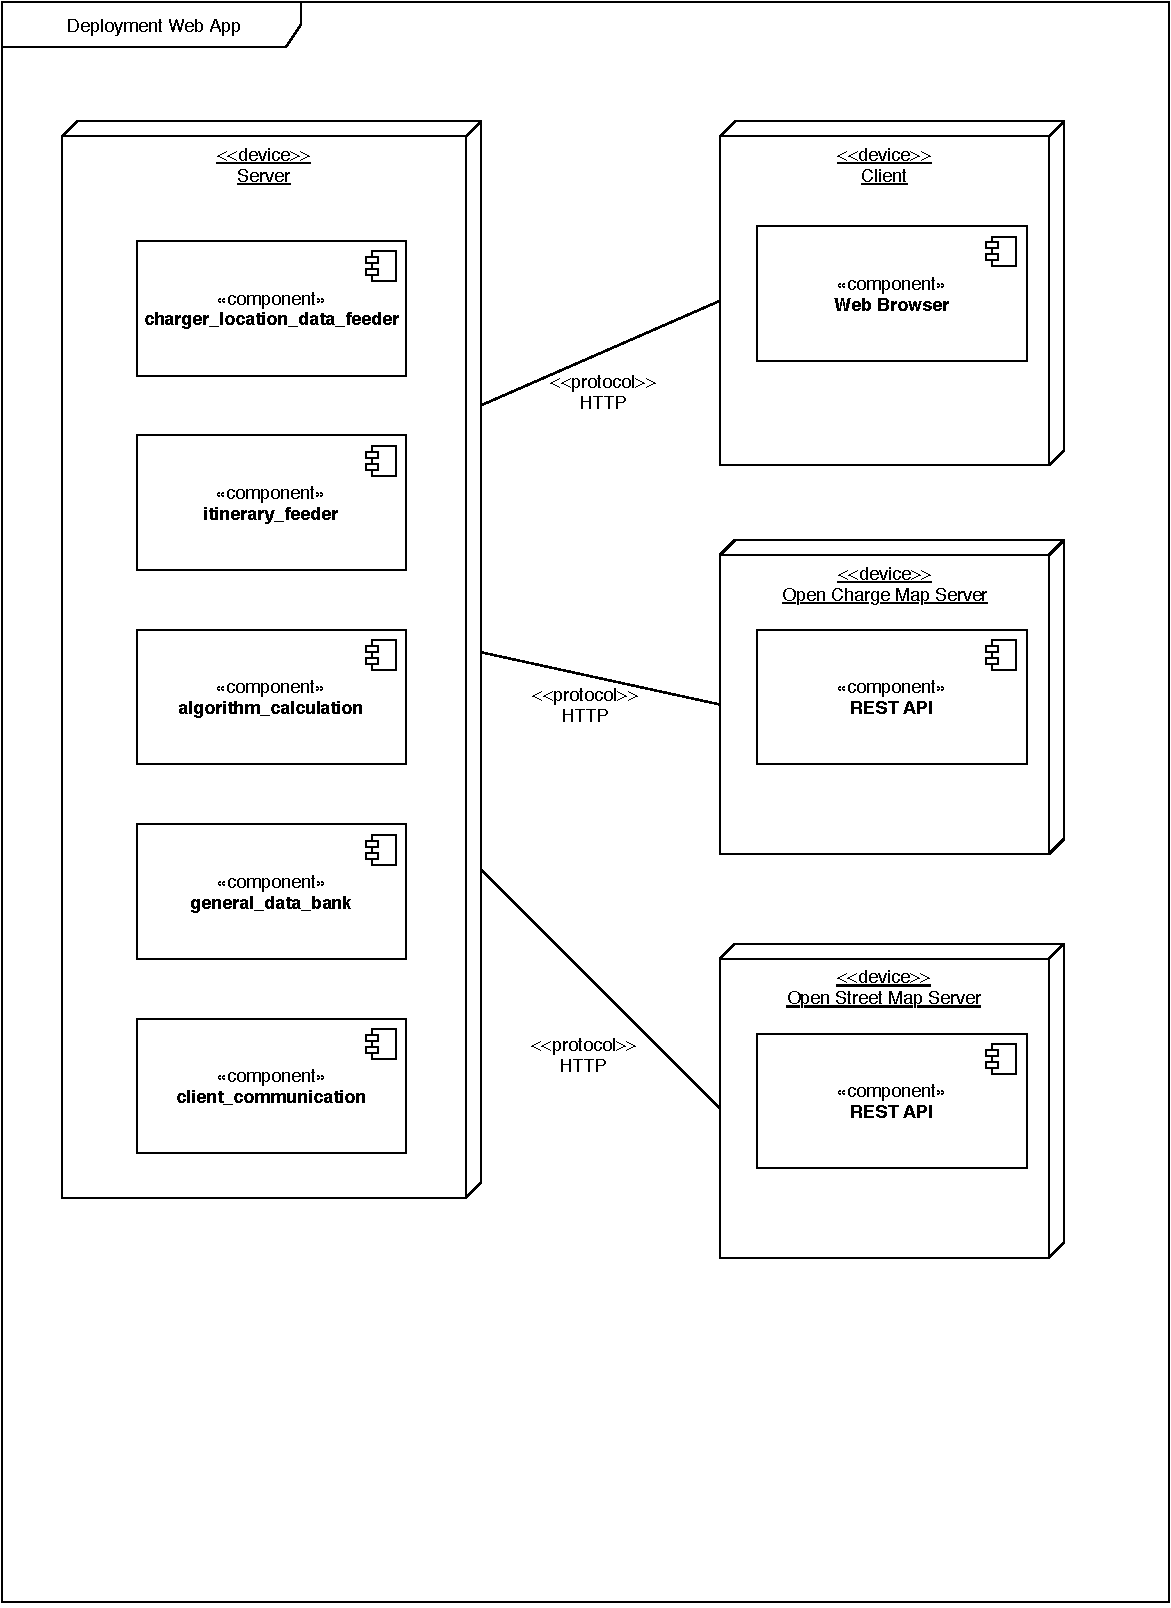
\includegraphics[scale=0.6]{Immagini/Deployment_Diagram.pdf}}
\caption{Deployment Diagram}
\end{figure}

\subsection{Architettura Hardware}

L'architettura che è emersa è ti tipo client-server a 2 livelli. Nel primo livello il client è impersonato dall'utilizzatore finale che richiede un servizio al nostro server attraverso il protocollo http. Nel secondo livello il nostro server recita la parte del client, richiedendo dei servizi alle due API a cui ci appoggiamo. (Figura 5.2 e Figura 5.3) \autocite[\protect\label{BassClementsKazman}][]{BassClementsKazman}

\begin{figure}[htp]
\centering
{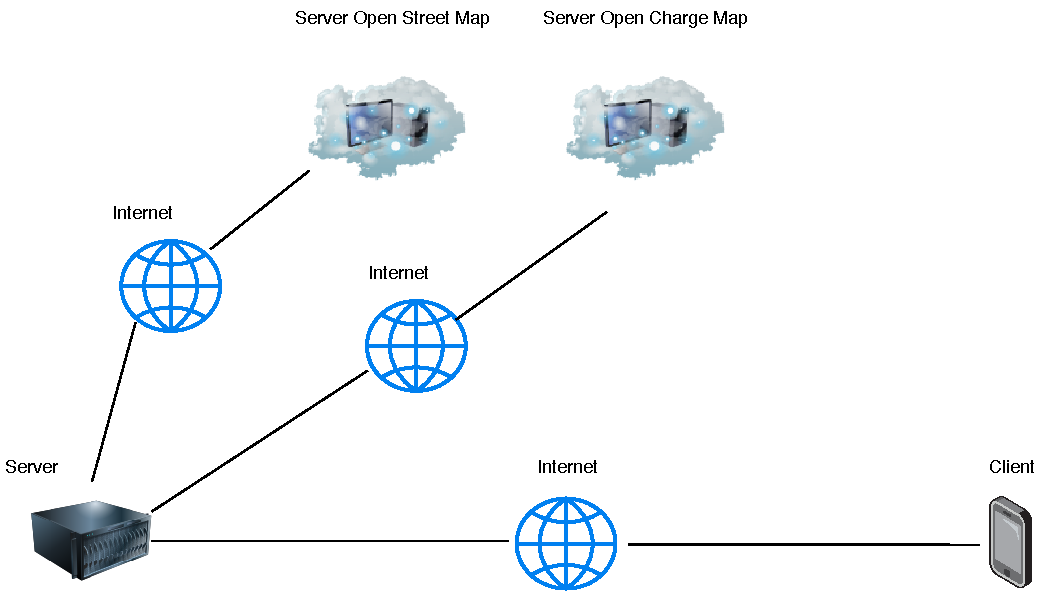
\includegraphics[scale=0.6]{Immagini/Architectural_Diagram.pdf}}
\caption{Architectural Diagram}
\end{figure}

\begin{figure}[htp]
\centering
{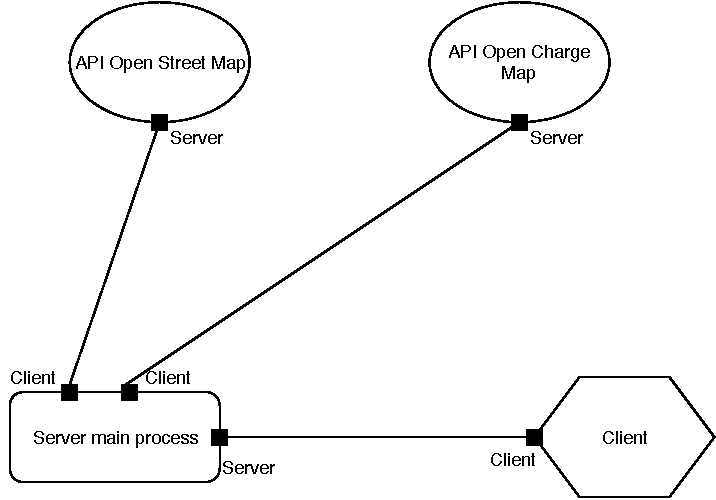
\includegraphics[scale=0.7]{Immagini/ClientServerArchitecture.pdf}}
\caption{Client-Server Architecture}
\end{figure}

\newpage

\section{Architettura Software}
L'archiettura software si divide in due diagrammi Component Diagram e Class Diagram.

\subsection{Component Diagram} \hypertarget{section::\theHsection}
Il diagramma delle componenti ha lo scopo di rappresentare la struttura interna del sistema software modellato in termini dei suoi componenti principali e delle relazioni fra di essi. (Figura 5.4)

\begin{figure}[htp]
\centering
{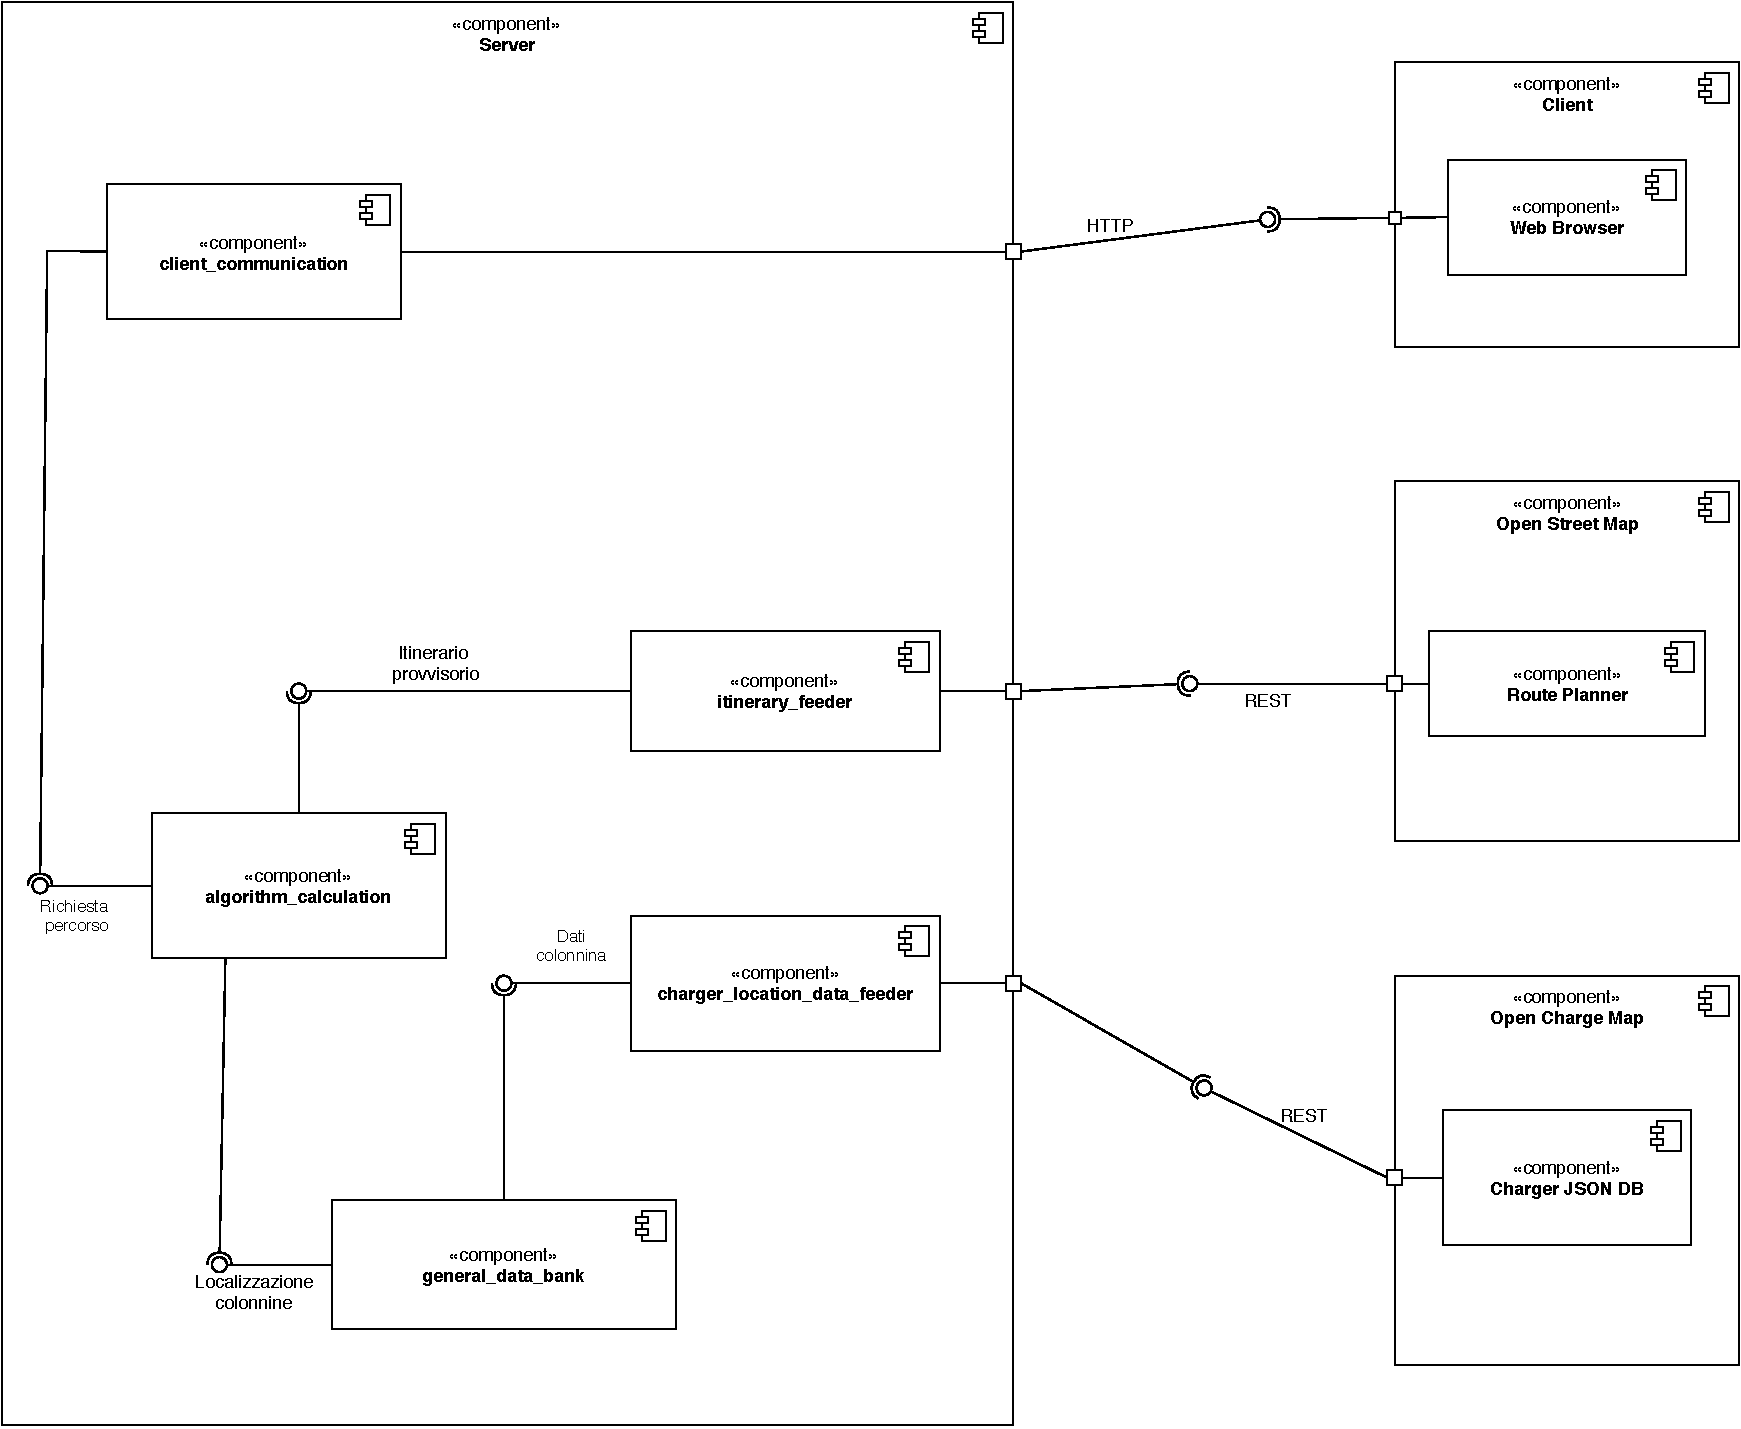
\includegraphics[scale=0.5]{Immagini/Component_Diagram.pdf}}
\caption{Component Diagram}
\end{figure}


\subsection{Class Diagram}
\hypertarget{section::\theHsection}
Il diagramma delle classi descrive il tipo degli oggetti che compongono il sistema e le relazioni statiche esistenti tra loro. (Figura 5.5)

\begin{figure}[htp]
\centering
{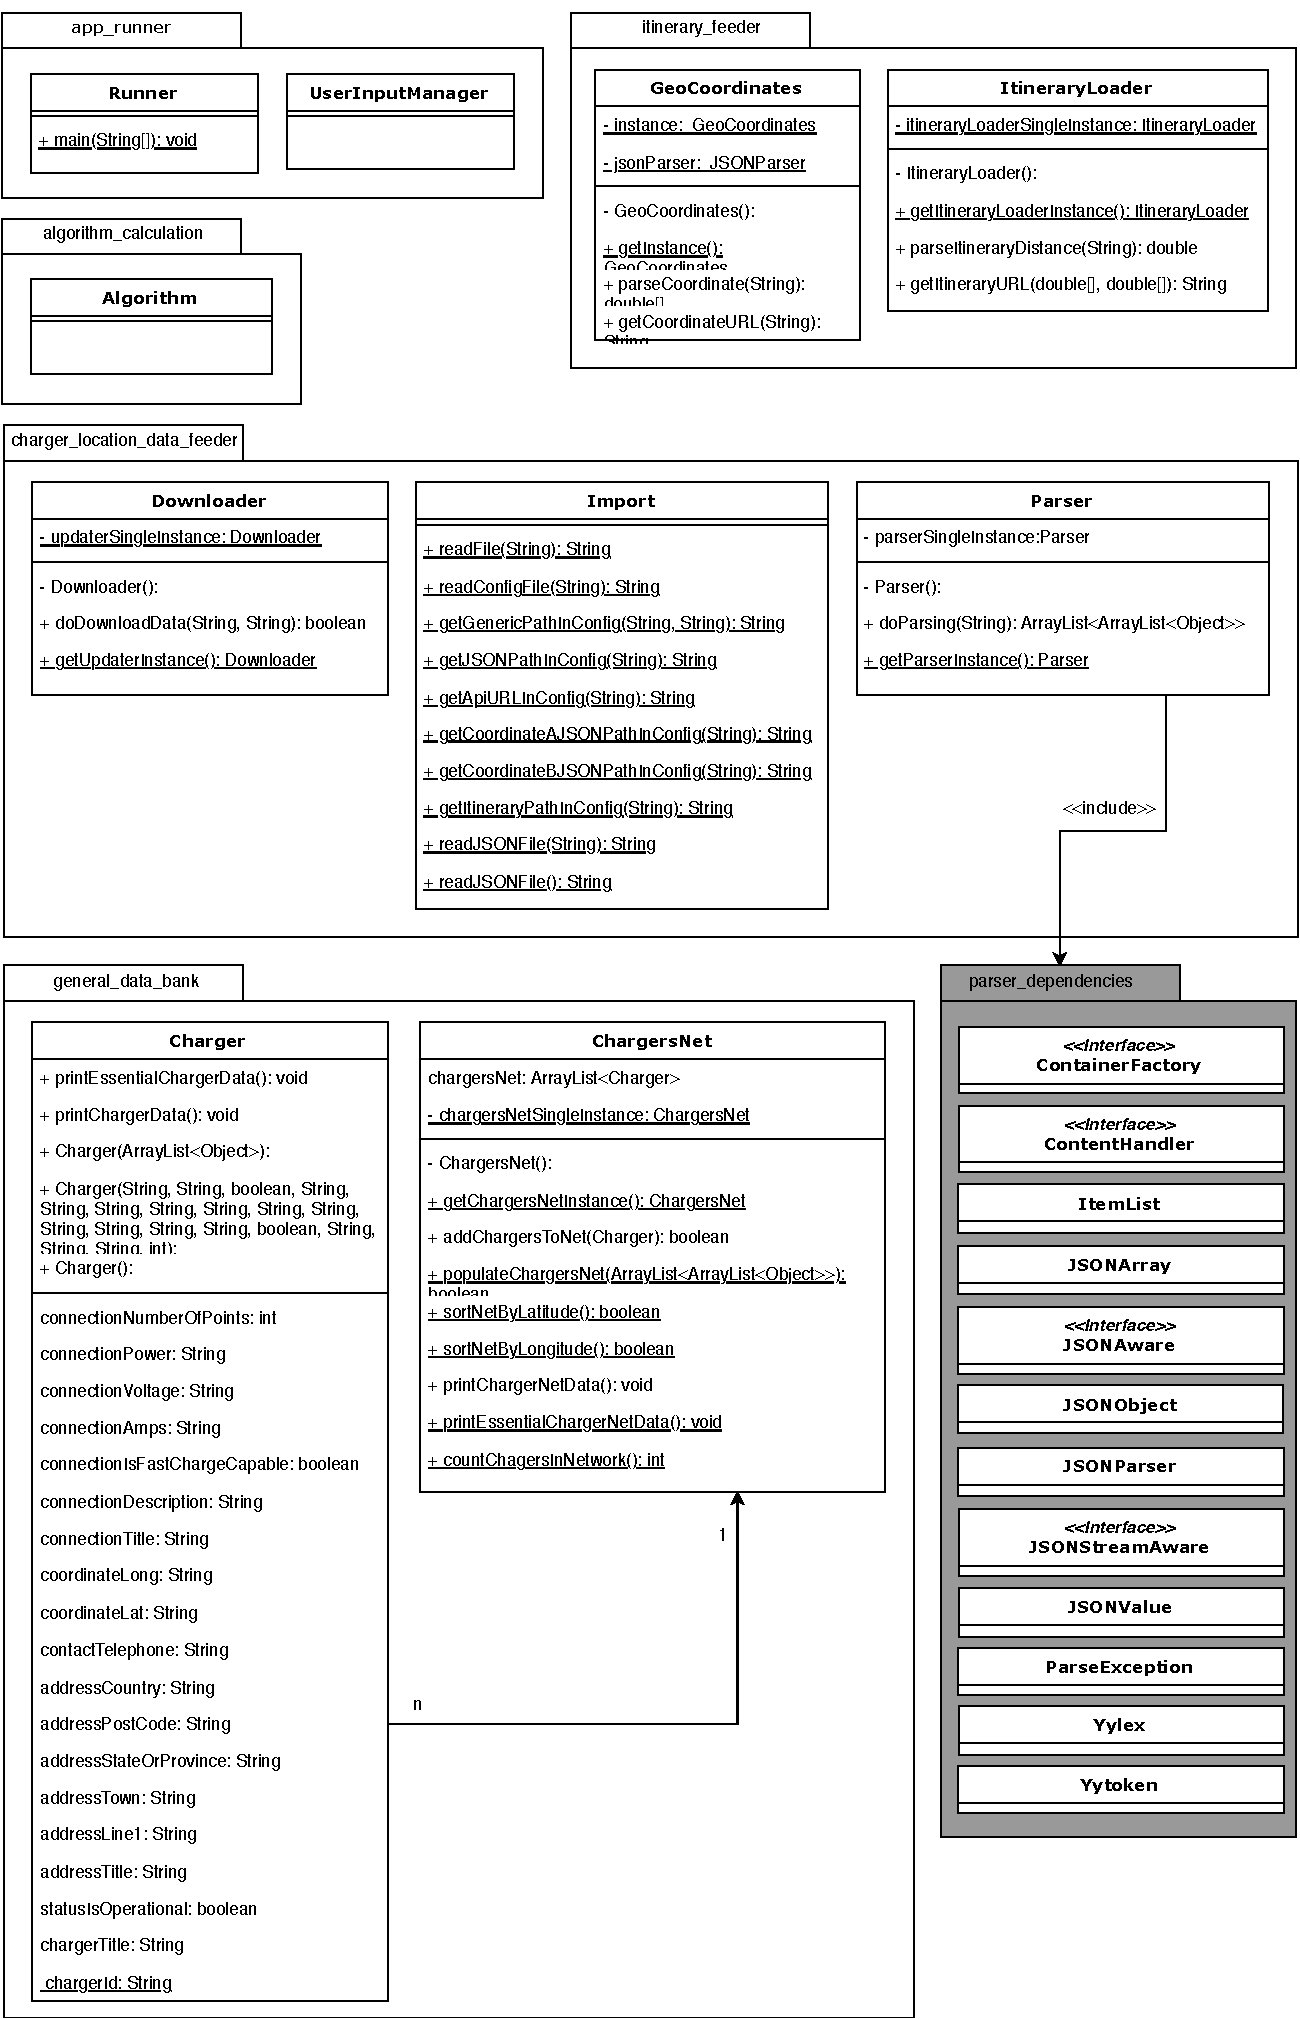
\includegraphics[scale=0.6]{Immagini/Class_Diagram.pdf}}
\caption{Class Diagram Architecture}
\end{figure}

\autocite[\protect\label{FerrariPighizzini2008}][]{FerrariPighizzini2008}

\part{Iterazione 1} \hypertarget{part::\theHpart}{}

\chapter{Parser}\label{chap:Parser} \hypertarget{chapter::\theHchapter}{}
\section {Scelta funzioni da implementare} \hypertarget{section::\theHsection}
Si è scelto di iniziare ad implementare le funzioni indispensabili del sistema da sviluppare tra cui la specifiche funzionali: R1, R6, R8 e i casi d'uso UC1 e UC2.

Per la parte di comunicazione tra l'applicazione e le API esterne, si è scelto di utilizzare il formato JSON, mentre per lo scaricamento e l'aggiornamento delle colonnine di ricarica viene usata una normale connessione http.

Lo scopo dell'applicazione é: date le colonnine di ricarica e il percorso da un punto A ad un punto B, essa calcolerà il percorso tenendo conto delle eventuali fermate per ricaricare l'auto.

I dati forniti all'algoritmo per l'elaborazione sono:
\begin{enumerate}
\item la posizione delle colonnine di ricarica
\item il percorso da un punto A ad un punto B
\end{enumerate}

Per la parte di comunicazione tra il nostro Server e le API è stato sviluppato un Parser che permette  una volta che il file viene scaricato dalle API di filtrarlo in base alle informazioni interessanti per il nostro progetto

\begin{center}
\textbf{\underline{INTERRUZIONE}}
\end{center}

Durante l'esecuzione di questa iterazione ci siamo resi conto che l'utilizzo del linguaggio Javascript per l'intero progetto avrebbe reso più agevole la realizzazione dello stesso. Abbiamo quindi deciso di interrompere questa iterazione e iniziare immediatamente la successiva dove illustreremo le modifiche effettuate all'iterazione 0 del processo.


\part{Iterazione 2} \hypertarget{part::\theHpart}{}

\chapter{Template HTML} \label{chap:Template HTML} \hypertarget{chapter::\theHchapter}{}
\section{Variazione linguaggio di programmazione } 
\hypertarget{section::\theHsection} 
Siccome per la parte di sviluppo della WebApp si è reso necessario utilizzare il linguaggio Javascript, la struttura e l'architettura del software sono state riviste al fine di utilizzare gli strumenti adatti allo sviluppo con tale linguaggio. Rimangono invariati rispetto a prima gli Use Cases, i requisisti funzionali del progetto e l'architettura hardware. Subisce invece variazioni l'architettura Software (deployment, component e class diagram). \autocite[\protect\label{BillNeil2009}][]{BillNeil2009}

\begin{figure}[htp]
\centering
{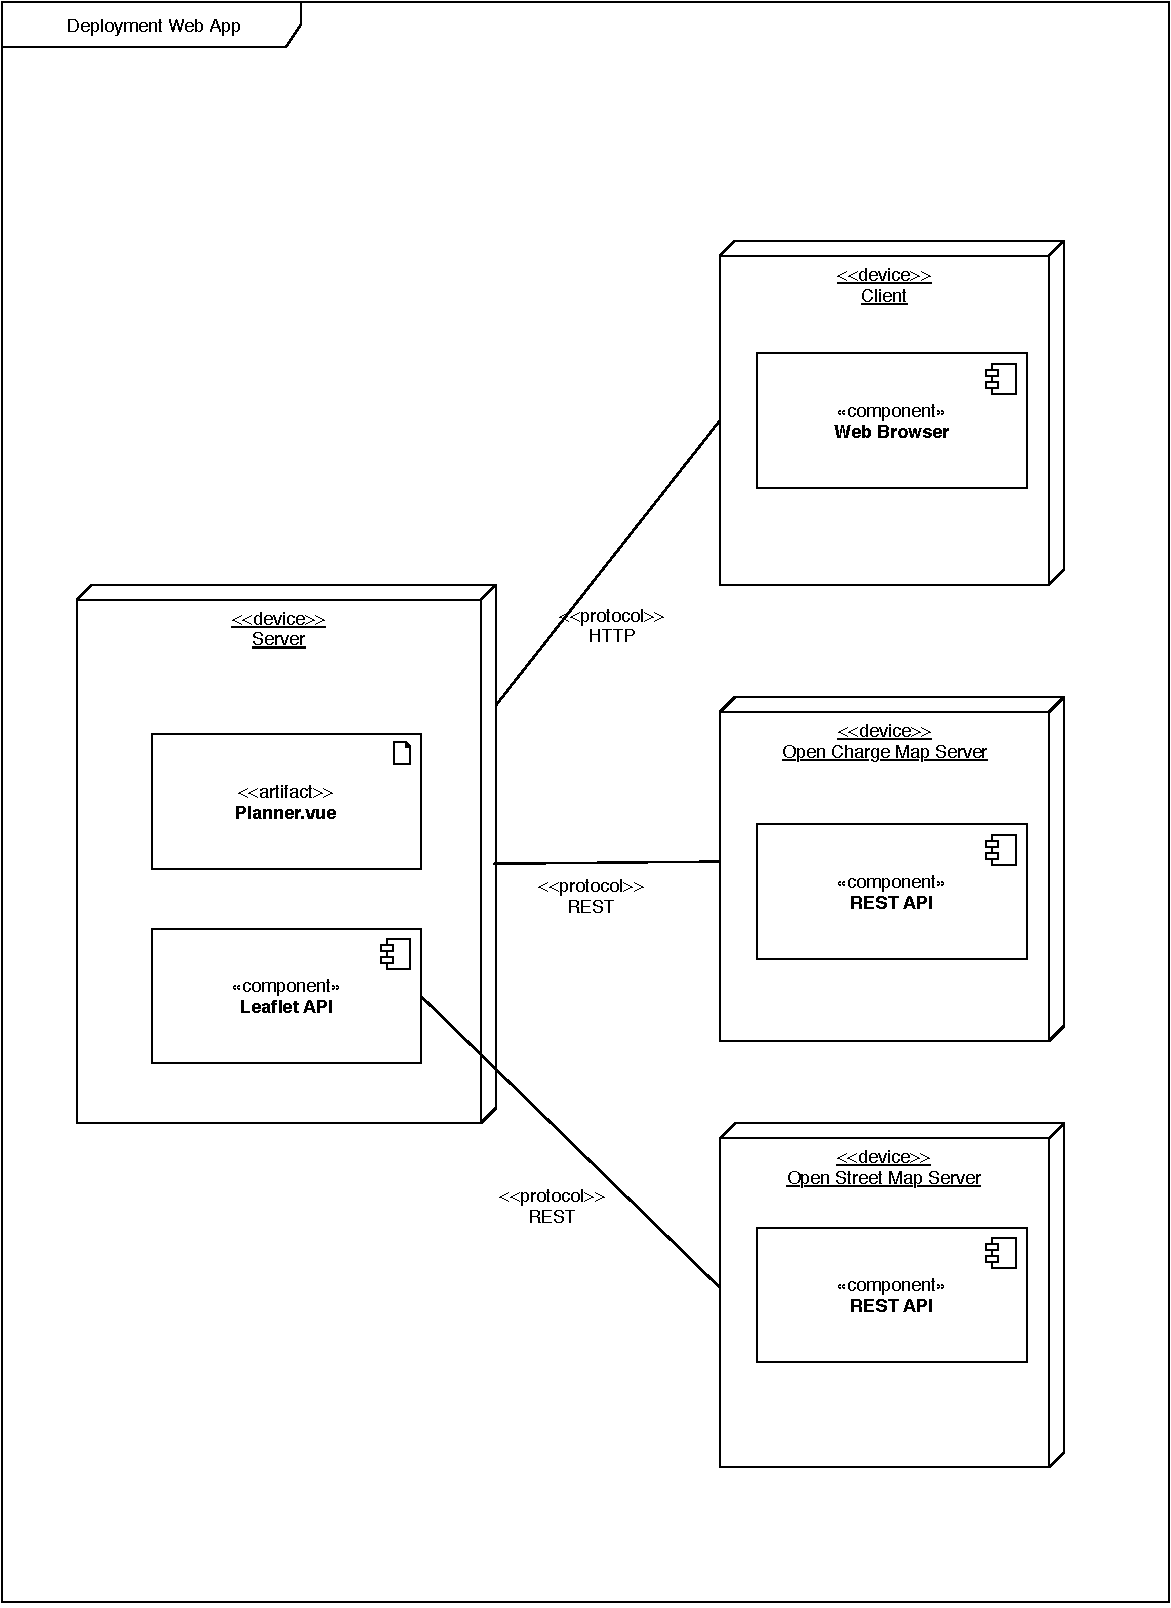
\includegraphics[scale=0.7]{Immagini/Deployment_Diagram_JS.pdf}}
\caption{Template Deployment Diagram}
\end{figure}

Il nuovo deployment diagram si presenta come mostrato in Figura 7.1. Sono presenti 4 device:

device Server che contiene il file Planner.vue che dovrà contenere il software sviluppato, la componente Leaflet API che avrà il compito di comunicare con le API di Open Street Map Server tramite protocollo REST.
Inoltre servirà utilizzare il device Open Charge Map Server e il device Client per lo scaricamento della posizione delle colonnine sulla mappa e la visualizzazione della WebApp sul pc come nel Deploy precedente.

\section {Template} \hypertarget{section::\theHsection}
Per lo sviluppo del software è stato sviluppato una parte di codice in HTML dove vengono definite le tre Textbox visualizzate a schermo, i due bottoni di Search e Reset e la visualizzazione della mappa a schermo centrata all'apertura sulla cartina geografica dell'Italia. \autocite[\protect\label{Sydik2007}][]{Sydik2007}

Per la parte puramente grafica invece è presente un CSS che inserisce nel sito gli elementi grafici visualizzati dall'utente che utilizza il software. \autocite[\protect\label{RobsonFreeman2012}][]{RobsonFreeman2012}

\section{Progettazione dei Test} 
\hypertarget{section::\theHsection}
Abbiamo provveduto alla progettazione dei test relativi a questa iterazione. Sappiamo che la nostra pagina web disporrà di campi in cui l'utente dovrà inserire dei valori e di pulsanti che potrà cliccare. Ci serve quindi un caso di test per questi elementi per assicurarsi che i valori inseriti vengano effettivamente ricevuti e che il click dei pulsanti chiami le relative funzioni: main() se viene cliccato il tasto "Search" e reset() se viene cliccato il tasto "Reset". \autocite[\protect\label{GoodmanMorrisonNovitskiRayl1996}][]{GoodmanMorrisonNovitskiRayl1996}


\section{Template Sequence Diagram}
\hypertarget{section::\theHsection}
Il diagramma di sequenza mostra come a partire da un attore, nel nostro caso un utente (User), il software evolve al fine di restituire all'utente un risultato che in questo caso specifico è rappresentato dalla visualizzazione su mappa del percorso con le fermate alle postazioni di ricarica.

Un utente inserisce l'url nel proprio Browser Web e questi restituirà l'Homepage del sito.
Una volta che l'utente inserisce i dati richiesti questi vengono inviati all'algoritmo scritto in Javascript, che a sua volta invierà una richiesta all'API Leaflet che avrà il compito di interrogare il database delle mappe di Open Street Map e restituire all'algoritmo il percorso dal punto di partenza a quello di destinazione.
L'algoritmo prenderà queste mappe e calcolerà quando è meglio fermarsi per ricaricare il veicolo elettrico, scegliendo tra le possibili colonnine sul percorso.
Dopodichè restituirà l'intero percorso dal punto di partenza a quello di destinazione all'utente con le eventuali fermate da effettuare. \autocite[\protect\label{RichardsonRuby2007}][]{RichardsonRuby2007}

\begin{figure}[H]
\centering
{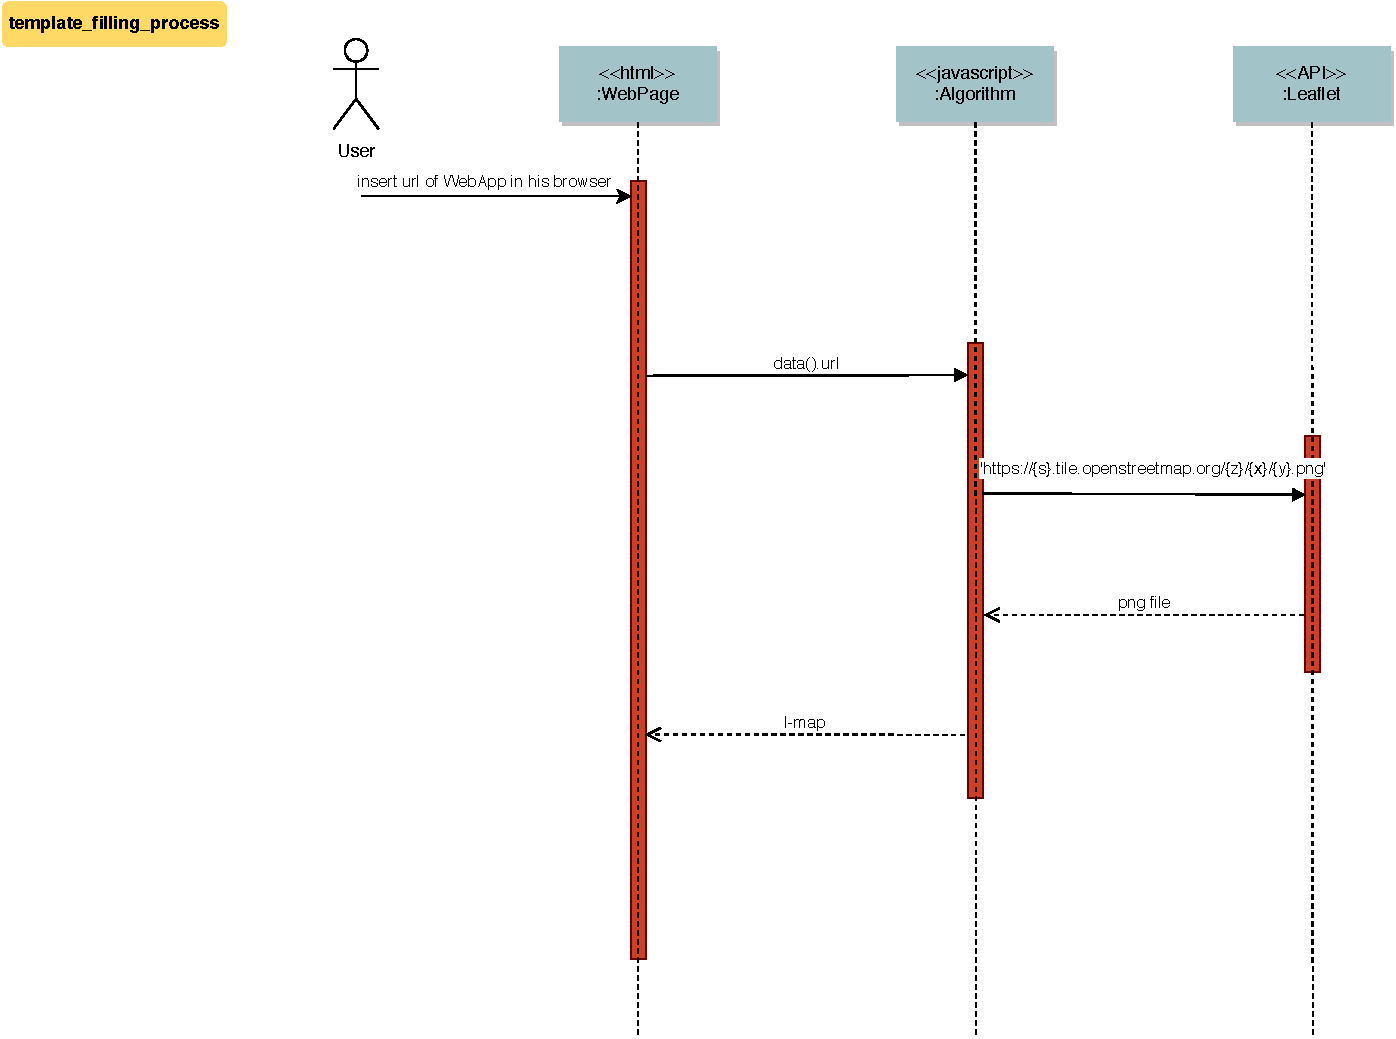
\includegraphics[scale=0.55]{Immagini/Template_SequenceDiagram.pdf}}
\caption{Template Sequence Diagram}
\end{figure}

\section{Risultato dei Test}
\hypertarget{section::\theHsection}
Per concludere questa iterazione presentiamo i risultati dei test che avevamo in precedenza definito. Come si può vedere dalla figura è stata eseguita una suite contente 4 test che hanno avuto tutti esito positivo.

\begin{figure}[H]
\centering
{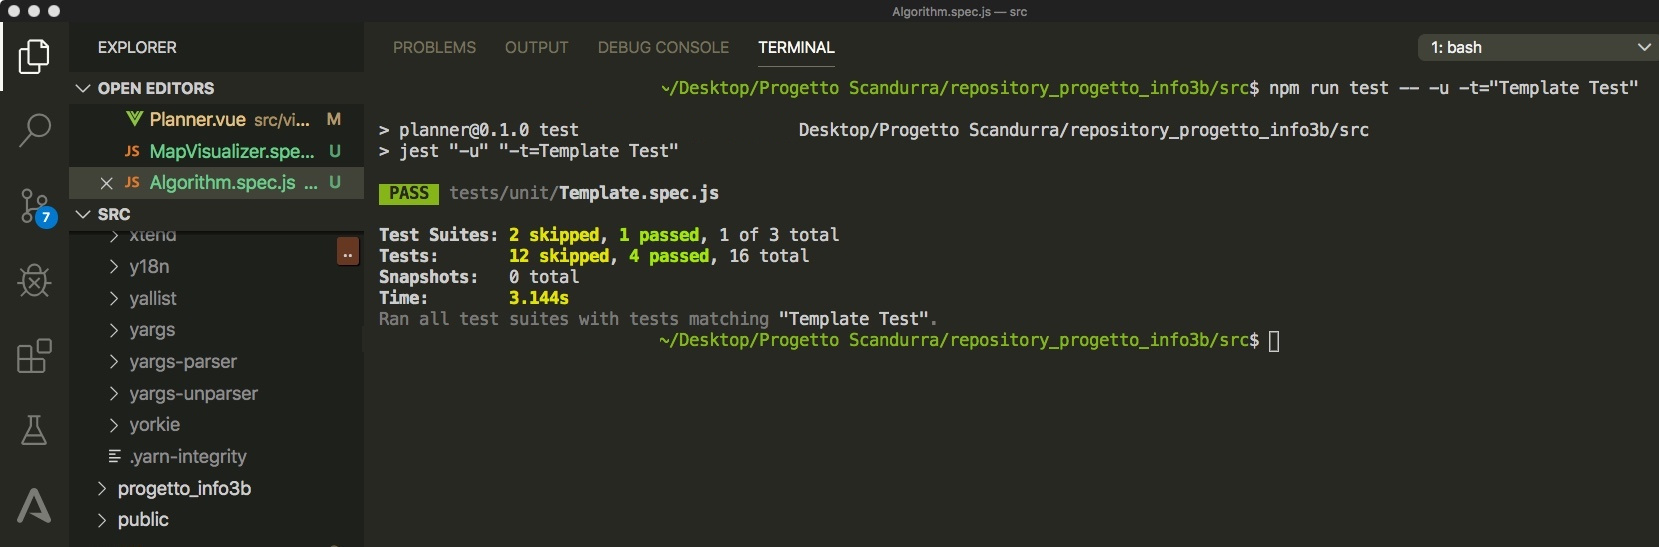
\includegraphics[scale=1]{Immagini/TestTemplate.jpeg}}
\caption{Test iterazione 2}
\end{figure}



\part{Iterazione 3} \hypertarget{part::\theHpart}{}

\chapter{Algoritmo} \label{chap:Algoritmo} \hypertarget{chapter::\theHchapter}{}
\section {Algoritmo e Flowchart}
\hypertarget{section::\theHsection}
In questo capitolo descriveremo i passi dell'algoritmo sviluppato. Essendo l'interazione complessa si è scelto di utilizzare un diagramma di flusso per dare una visione generale di più immediata comprensione.
Il flowchart completo di tutto l'algoritmo è mostrato in Figura 8.1

\begin{figure}[htp]
\centering
{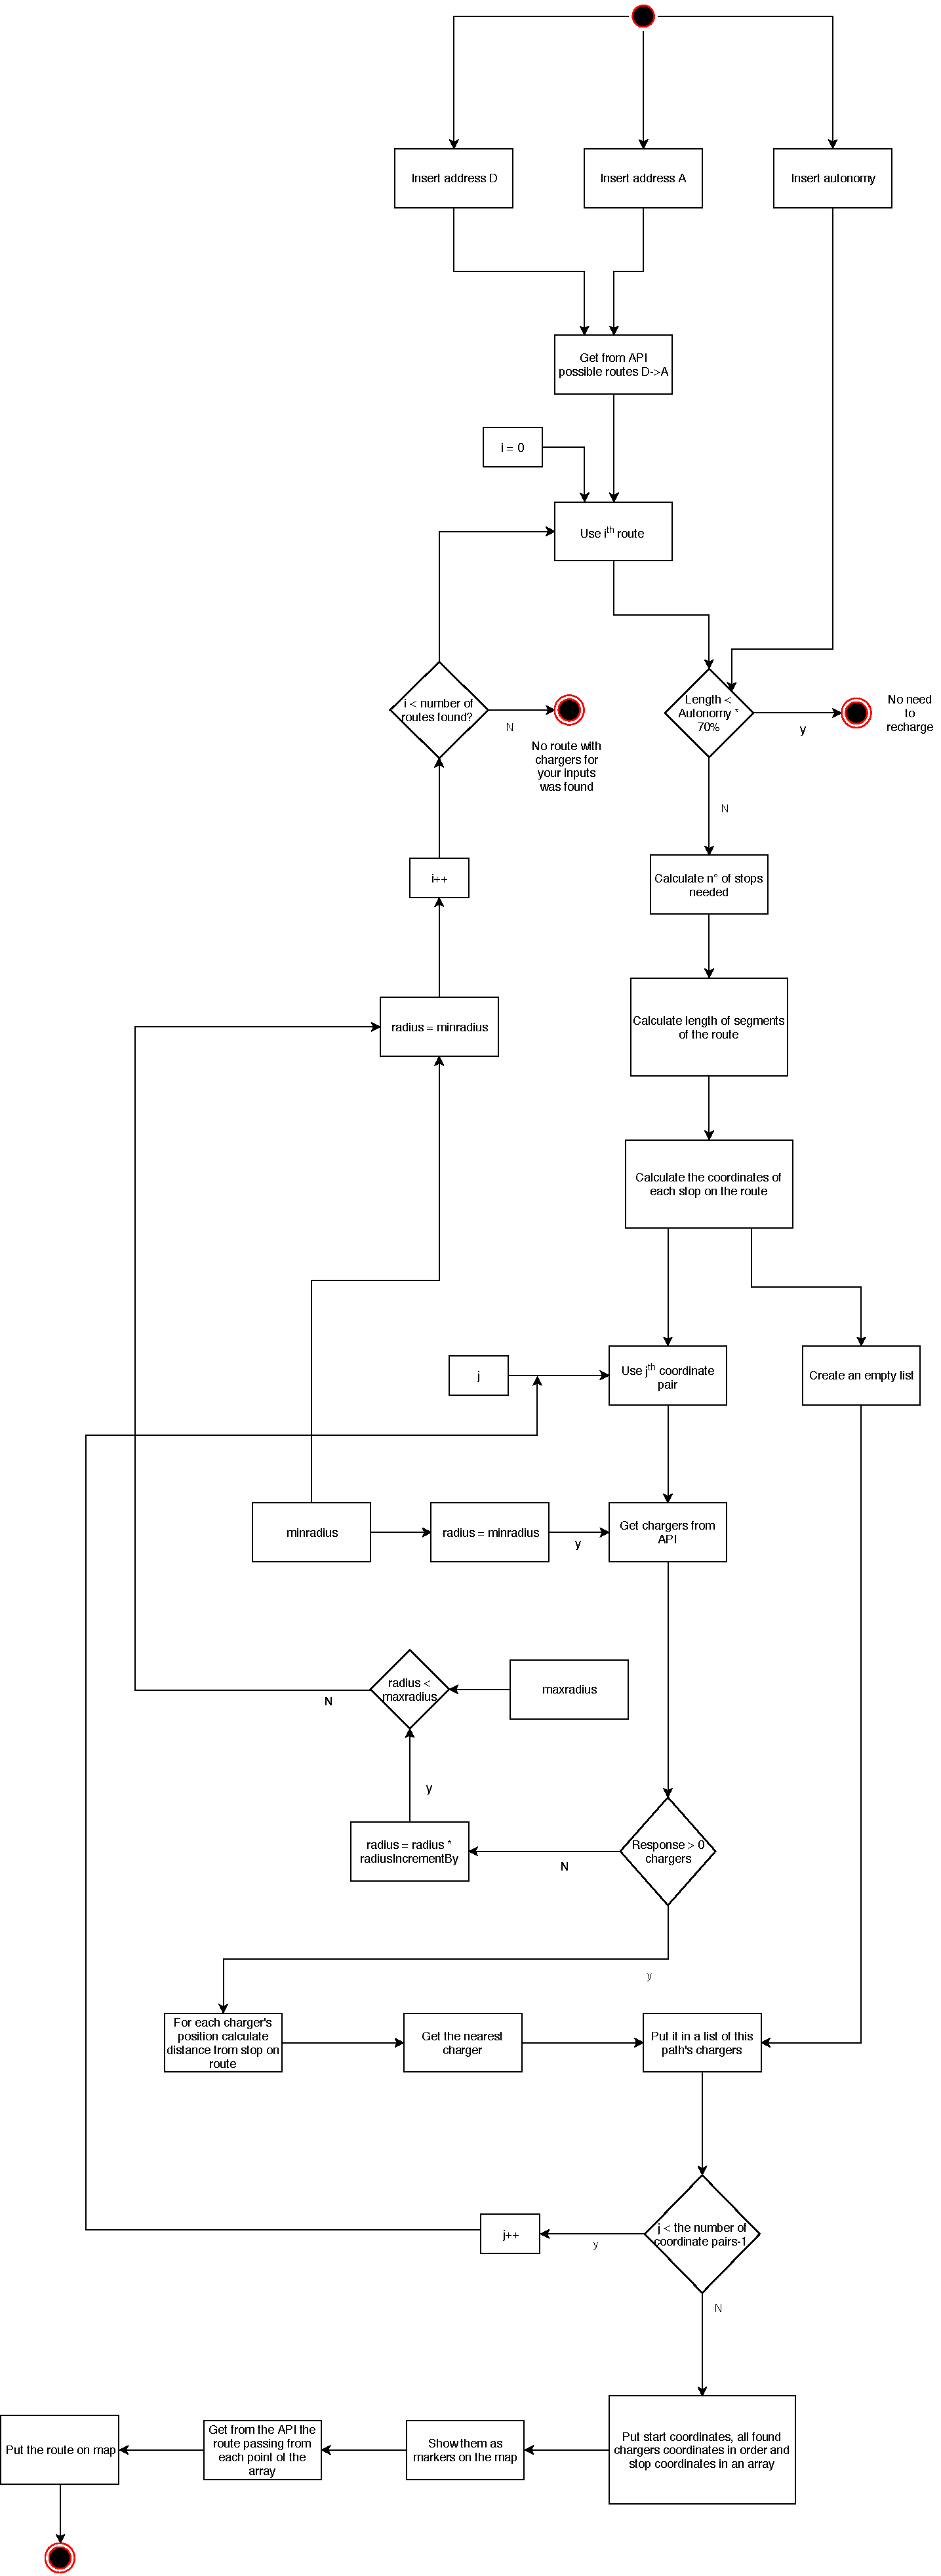
\includegraphics[scale=0.30]{Immagini/Algoritmo_Flowchart.pdf}}
\caption{Flowchart Algorithm}
\end{figure}

\subsection{Analisi di complessità}
\hypertarget{section::\theHsection}
Procediamo ora all'analisi di complessità dell'algoritmo. Per cercare di analizzarlo risulta utile avere un'idea più chiara e di alto livello su ciò che l'algoritmo effettivamente fa; una spiegazione testuale può quindi risultare utile.
L'esecuzione inizia richiedendo a OpenStreetMap il percorso fra il punto di partenza e il punto di arrivo inseriti dall'utente. L'API restituisce tutti i percorsi che è riuscita a trovare in ordine ottimale, ossia in ordine crescente di tempo di percorrenza. E' importante notare, per il proseguo della spiegazione, che i percorsi vengono forniti come una serie di punti adiacenti. A questo punto subentra l'algoritmo vero e proprio che analizza i percorsi nell'ordine in cui gli sono stati forniti, attraverso la funzione \textit{getStopCircleCenterPoints}, nel seguente modo: partendo dal punto iniziale si sommano le distanze (che vanno calcolate), fra i punti che costituiscono il percorso fino a raggiungere una distanza maggiore dell'autonomia dichiarata dall'utente. A questo punto si torna indietro di un punto e lo si aggiunge all'array di punti dove sarà necessario fermarsi. Alla fine di quest'analisi si ha quindi la lista delle coordinate nei pressi delle quali è necessario fermarsi. Viene quindi chiamata la funzione \textit{obtainChargersForThisRoute} la quale, insieme alla funzione \textit{getSmallestElementsIndex}, trova il charger più vicino. La ricerca del charger avviene nel seguente modo: viene definito un cerchio di raggio 1 centrato nel punto trovato in precedenza e si cerca in quest'area il charger più vicino. Nel caso non venisse trovato alcun charger si estende incrementalmente il raggio del cerchio fino ad un massimo di \[maxRadius = \frac{1 - batteryPercentageUsage}{2} * Autonomia\] Le coordinate del charger trovato vengono inserite nel percorso e questo viene conseguentemente modificato per includere il passaggio per la colonnina di ricarica. Nel caso in cui non sia possibile trovare un charger per anche solo uno dei punti in cui è necessario fermarsi, il percorso viene dichiarato invalido e l'algoritmo procede ad esaminare il successivo risultato fornitogli dall'API.
E' quindi possibile notare che l'algoritmo è costituito da una prima parte di programmazione dinamica, in cui si calcola la somma delle distanze fra tutti i punti successivi, e una seconda parte di stampo greedy, in cui si cerca la soluzione (charger) ottima più vicina, allargando mano a mano l'insieme dei candidati non ancora esplorati. \autocite[\protect\label{BertossiMontresor2000}][]{BertossiMontresor2000}

E' ora possibile analizzare la complessità dell'algoritmo: la parte dinamica si basa sulla somma degli n segmenti che costituiscono il percorso, e può quindi essere portata a termine in tempo $O(n)$.
La seconda parte greedy viene eseguita nel seguente modo: l'algoritmo riceve la lista dei charger presenti nell'area e calcola la distanza di ciascuno di essi dal centro del cerchio, quindi seleziona il charger con distanza minore. Dato \textit{m} il numero di charger restituiti dall'API per quell'area, l'operazione è semplicemente il calcolo della distanza e viene quindi espletata in tempo $O(m)$. Siccome il numero di charger restituiti è generalmente piccolo, l'operazione può essere eseguita in un tempo costante $\Theta(1)$. Si nota inoltre che la funzione per trovare i charger viene chiamata un numero costante di volte (molto inferiore a n), quindi l'intera operazione è $\Theta(1)$. Da ciò ne deriva che il tempo totale di esecuzione dell'algoritmo è dato solo dalla parte di calcolo delle somme delle distanze ed è perciò $O(n)$.

\subsection{Pseudocodice}
\hypertarget{section::\theHsection}
Segue lo pseudocodice.

\lstinputlisting[language=JavaScript]{Codice/pseudocode_importLibraries.pseudo}

\lstinputlisting[language=JavaScript]{Codice/pseudocode_data.pseudo}

\lstinputlisting[language=JavaScript]{Codice/pseudocode_main.pseudo}

\lstinputlisting[language=JavaScript]{Codice/pseudocode_handleRoutesFound.pseudo}

\lstinputlisting[language=JavaScript]{Codice/pseudocode_obtainChargersForThisRoute.pseudo}

\lstinputlisting[language=JavaScript]{Codice/pseudocode_calculateDistancesFromRouteCoordinates.pseudo}

\lstinputlisting[language=JavaScript]{Codice/pseudocode_getStopCircleCenterPoints.pseudo}

\lstinputlisting[language=JavaScript]{Codice/pseudocode_getSmallestElementsIndex.pseudo}

\lstinputlisting[language=JavaScript]{Codice/pseudocode_displayResults.pseudo}

\subsection{Diagrammi di attività}
\hypertarget{section::\theHsection}
Il diagramma di sequenza è mostrato in Figura 8.2 questo diagramma mostra come le varie componenti interagiscono tra di loro e i dati che si scambiano.


\begin{figure}[H]
\centering
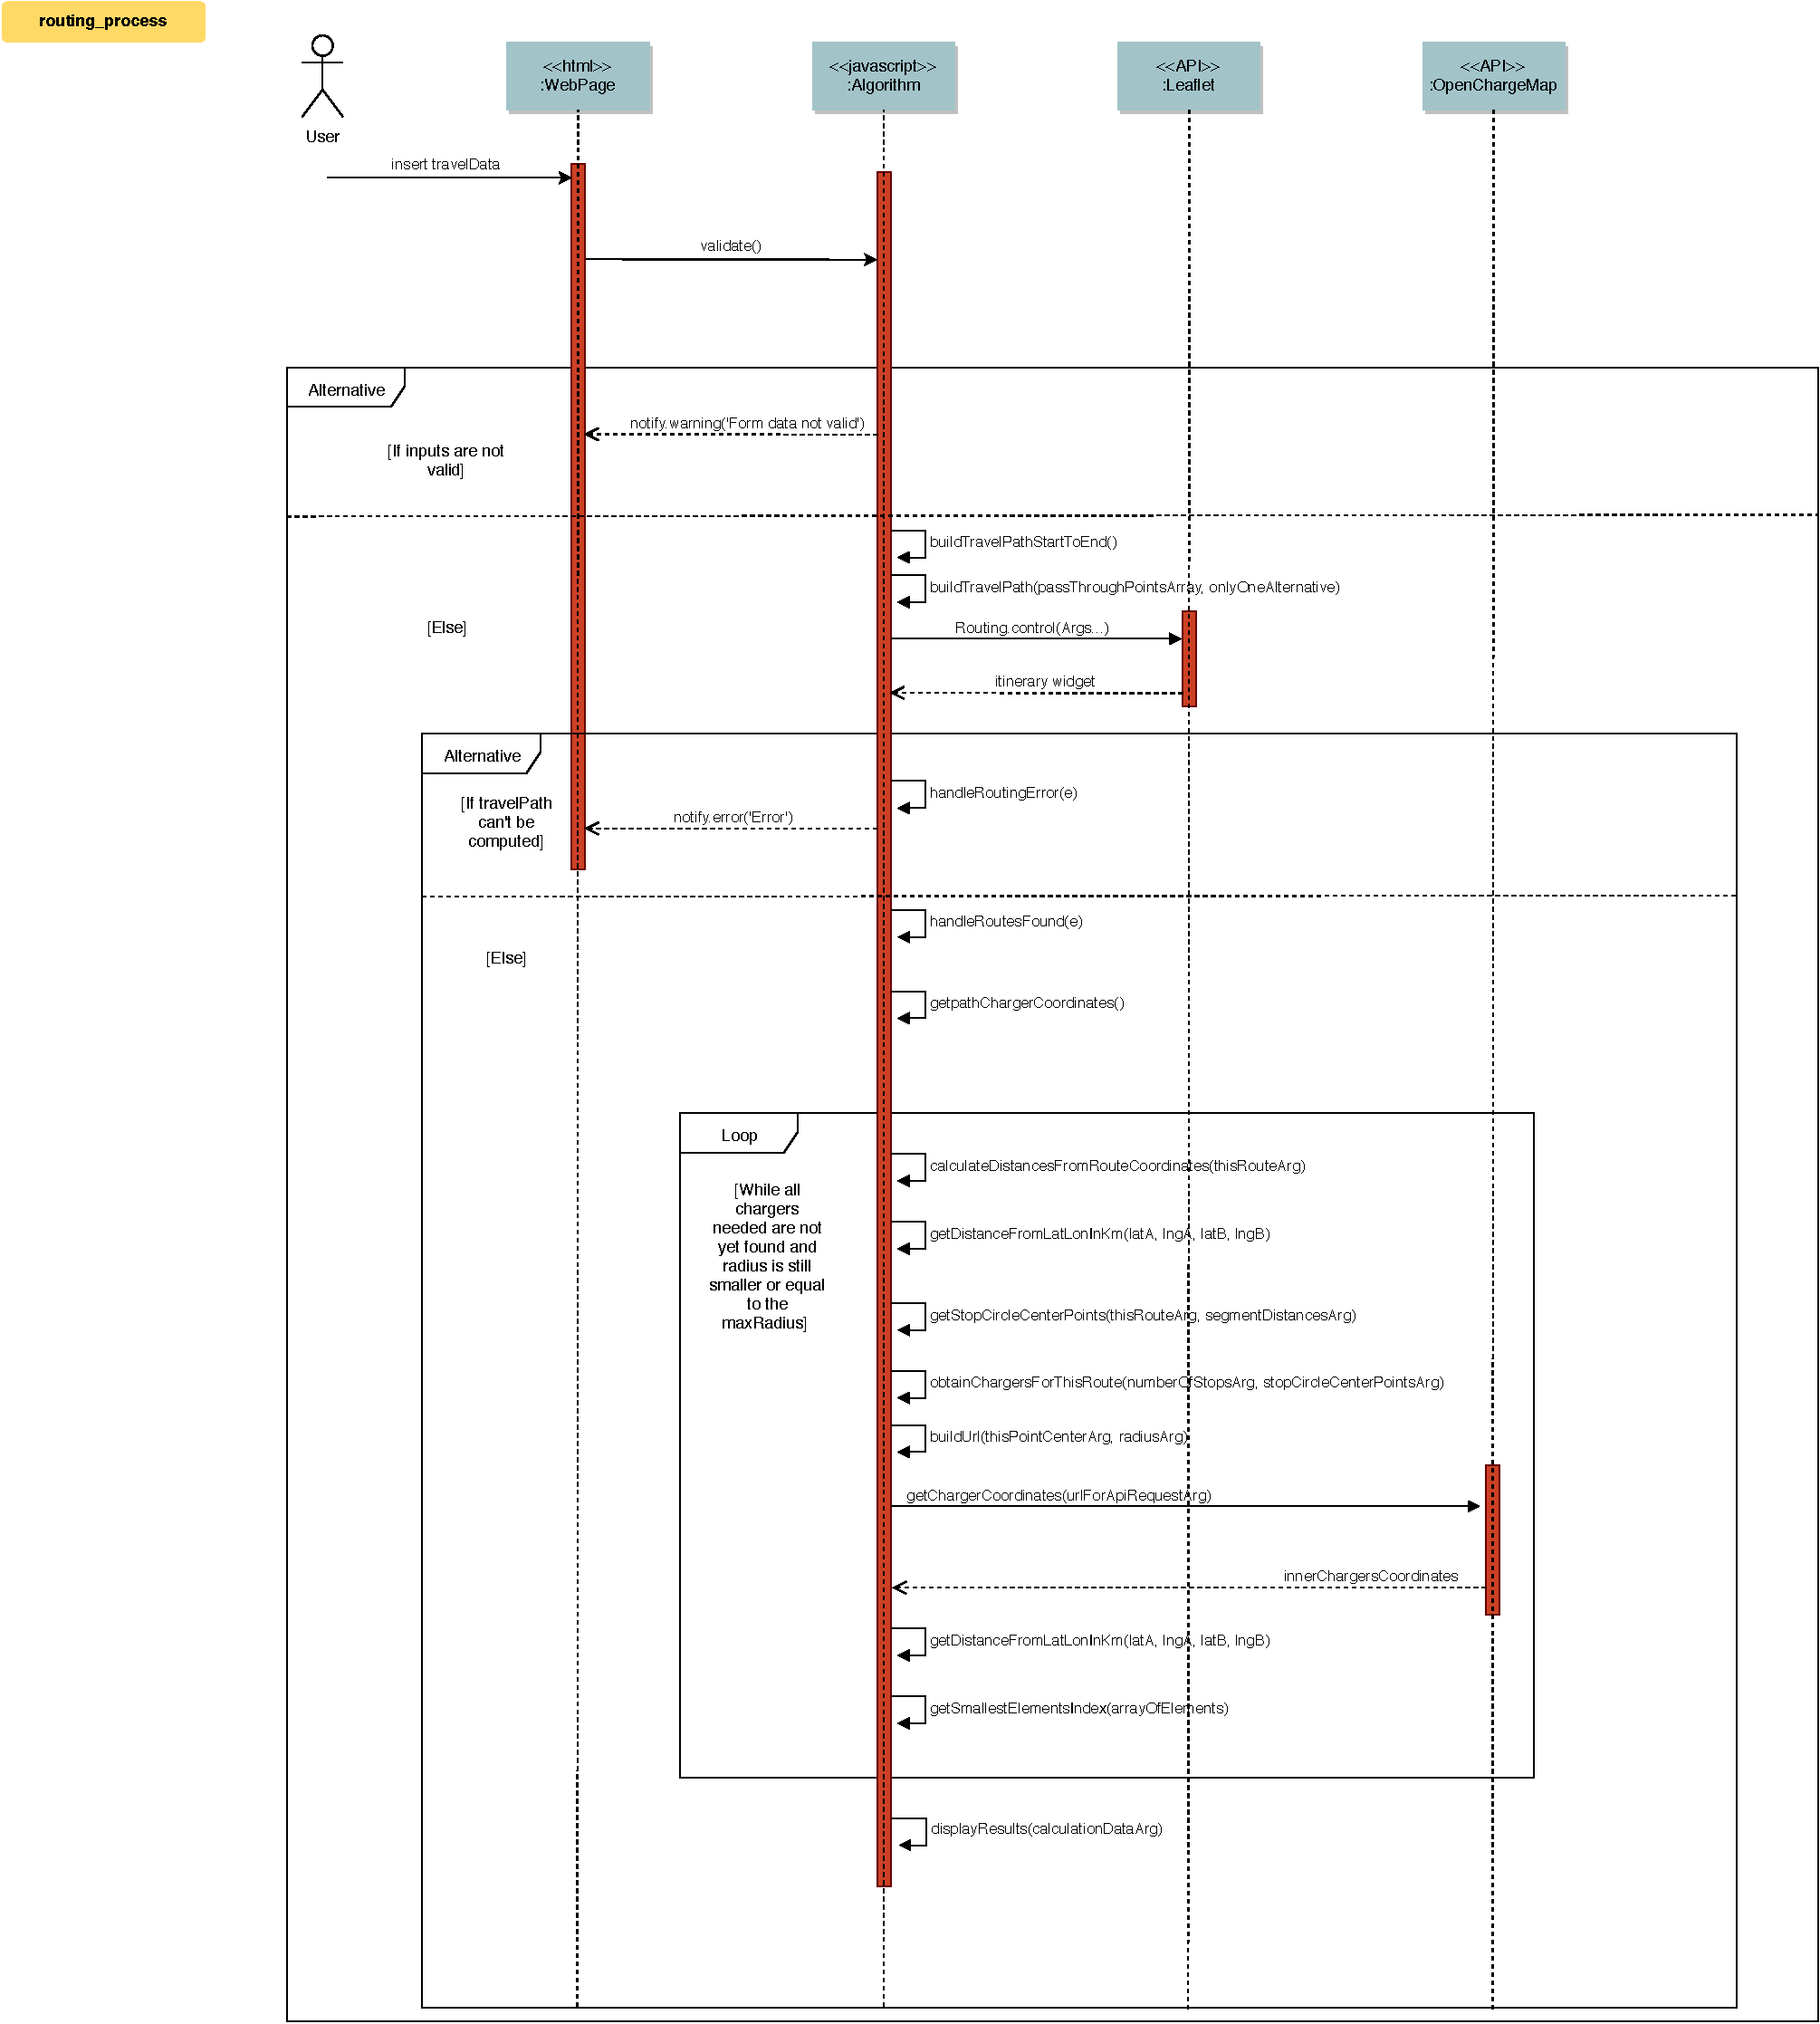
\includegraphics[scale=0.4]{Immagini/Algorithm_SequenceDiagram.pdf}
\caption{Algorithm Sequence Diagram}
\end{figure}

Nella Figura 8.3 sono mostrati, più in dettaglio, i metodi e le relative chiamate che l'algoritmo utilizza per la sua computazione.

\begin{figure}[htp]
\centering
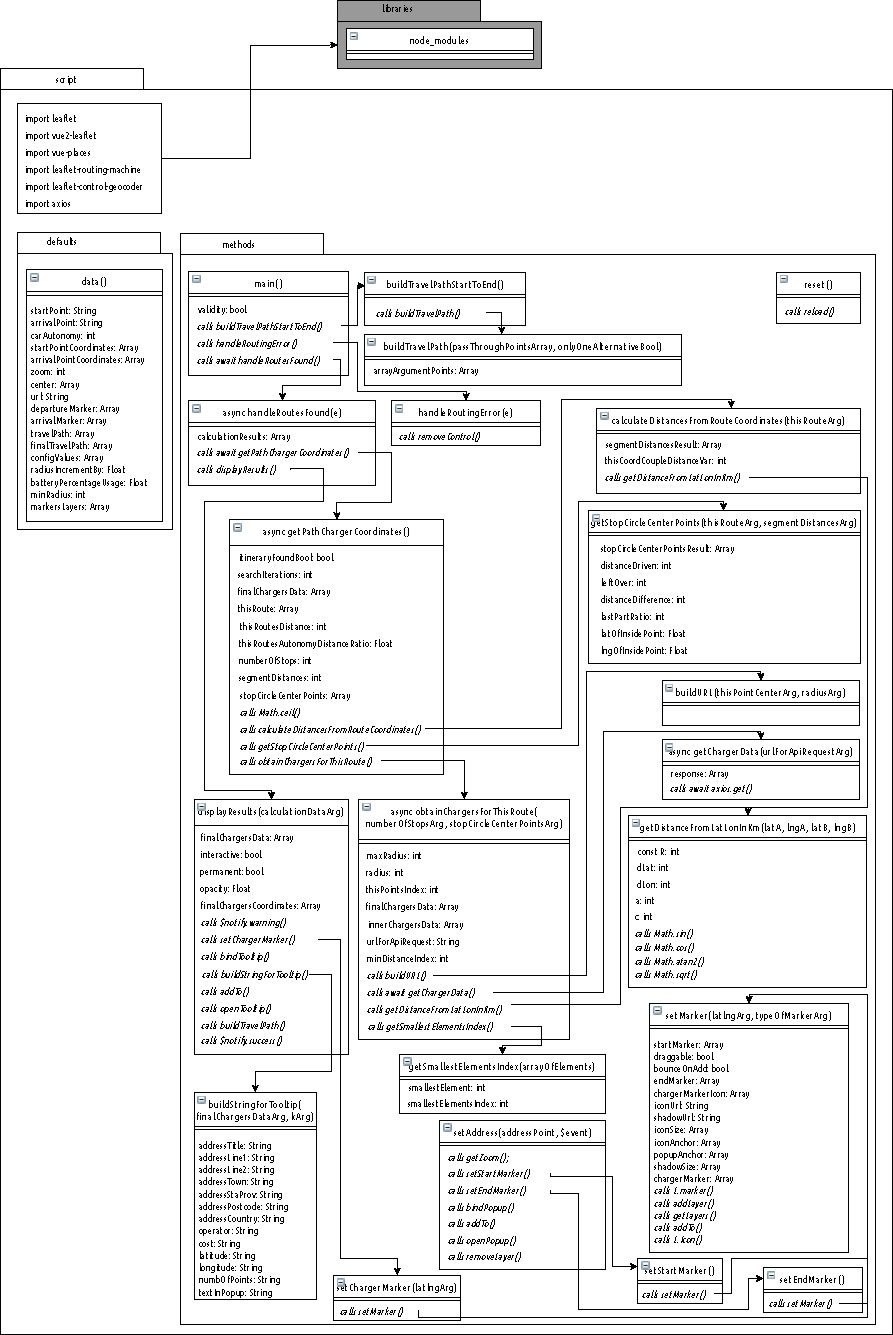
\includegraphics[scale=0.9]{Immagini/Methods_Diagram.pdf}
\caption{Methods}
\end{figure}

\section{Progettazione dei Test} 
\hypertarget{section::\theHsection}
L'algoritmo che abbiamo progettato è costituito da diverse funzioni. Per verificarne il comportamento testeremo queste funzioni controllando che i parametri passati e i valori restituiti coincidano con quanto ci aspettiamo. In particolare testeremo le funzioni riportate in tabella 8.1 .

\begin{table}[h]
\centering
\begin{tabular}{|c|l|c|}
\hline
Funzione                  & Descrizione                                                                                                                                      & Esito test \\ \hline
setMarker                 & aggiunge un Marker alla lista                                                                                                                    & Passato    \\ \hline
setChargerMarker          & aggiunge un Marker per un charger                                                                                                                & Passato    \\ \hline
setStartMarker            & aggiunge il Marker per il punto di partenza                                                                                                      & Passato    \\ \hline
setEndMarker              & aggiunge il Marker per il punto di arrivo                                                                                                        & Passato    \\ \hline
buildStringForTooltip     & \begin{tabular}[c]{@{}l@{}}costruisce la stringa da visualizzare a schermo \\ riportante le informazioni circa il punto di ricarica\end{tabular} & Passato    \\ \hline
getSmallestElementsIndex  & ottiene l'indice del charger più vicino al punto selezionato                                                                                     & Passato    \\ \hline
buildUrl                  & \begin{tabular}[c]{@{}l@{}}costruisce l'URL per effettuare la richiesta all'API \\ di Open Charge Map\end{tabular}                               & Passato    \\ \hline
getStopCircleCenterPoints & \begin{tabular}[c]{@{}l@{}}calcola il punto lungo il tragitto in cui è necessario\\  fermarsi per la ricarica\end{tabular}                       & Passato    \\ \hline
getDistanceFromLatLonInKm & calcola la distanza fra due punti                                                                                                                & Passato    \\ \hline
\end{tabular}
\caption{Funzioni implementate nella suite di test}
\end{table}


\section{Risultato dei Test} 
\hypertarget{section::\theHsection}
Il risultato dei test eseguiti è riportato nella figura qui sotto. E' stata eseguita una suite composta di nove test che hanno ricevuto esito positivo.

\begin{figure}[htp]
\centering
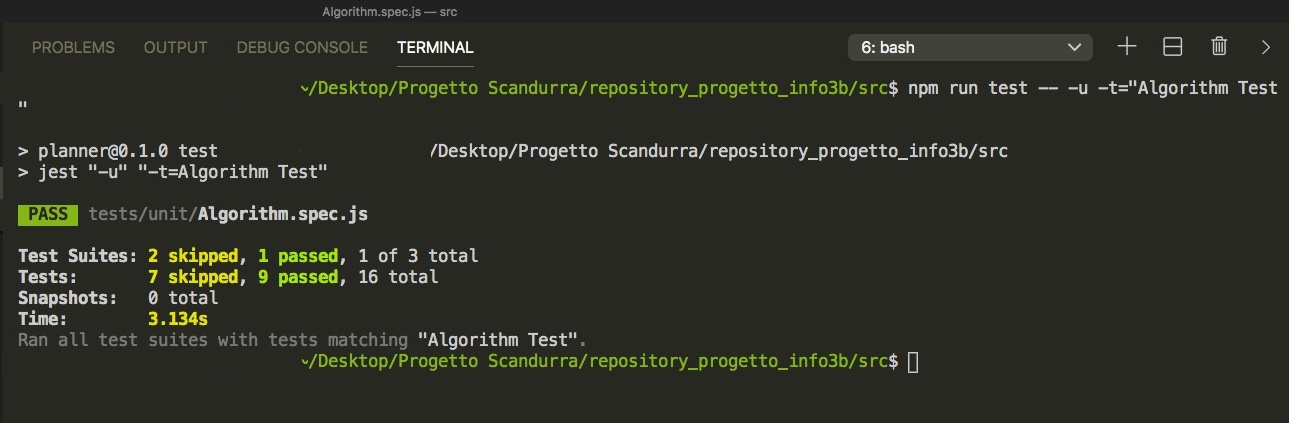
\includegraphics[scale=1.3]{Immagini/TestAlgorithm.jpeg}
\caption{Test iterazione 3}
\end{figure}

E' quindi possibile passare all'ultima iterazione del nostro processo AMDD.

\part{Iterazione 4} \hypertarget{part::\theHpart}{}

\chapter{Visualizzazione Percorso} \label{chap:Visualizzazione Percorso} \hypertarget{chapter::\theHchapter}{}
In questa ultima sezione ci occupiamo di progettare la parte del software che permetterà la visualizzazione del percorso (calcolato in precedenza), sulla mappa, con le eventuali fermate da effettuare.

\section{Progettazione dei Test} 
\hypertarget{section::\theHsection}
Sappiamo che la funzione che si occuperà di disegnare il tragitto dovrà prendere in input le coordinate dei punti di sosta, creare i marker sulla mappa, tracciare il percorso e restituire un valore booleano. Sappiamo inoltre che all'interno di questa funzione ci saranno diversi \textit{if statements}, quindi ci assicuriamo di testare le varie casistiche che si svilupperanno in fase di esecuzione.

\section{Pseudocodice} 
\hypertarget{section::\theHsection}
Di seguito è riportato in pseudocodice la parte di visualizzazione del percorso sulla mappa. \autocite[\protect\label{Zammetti2007}][]{Zammetti2007}
\lstinputlisting[language=JavaScript]{Codice/pseudocode_displayResults.pseudo}

\begin{figure}[htp]
\centering
{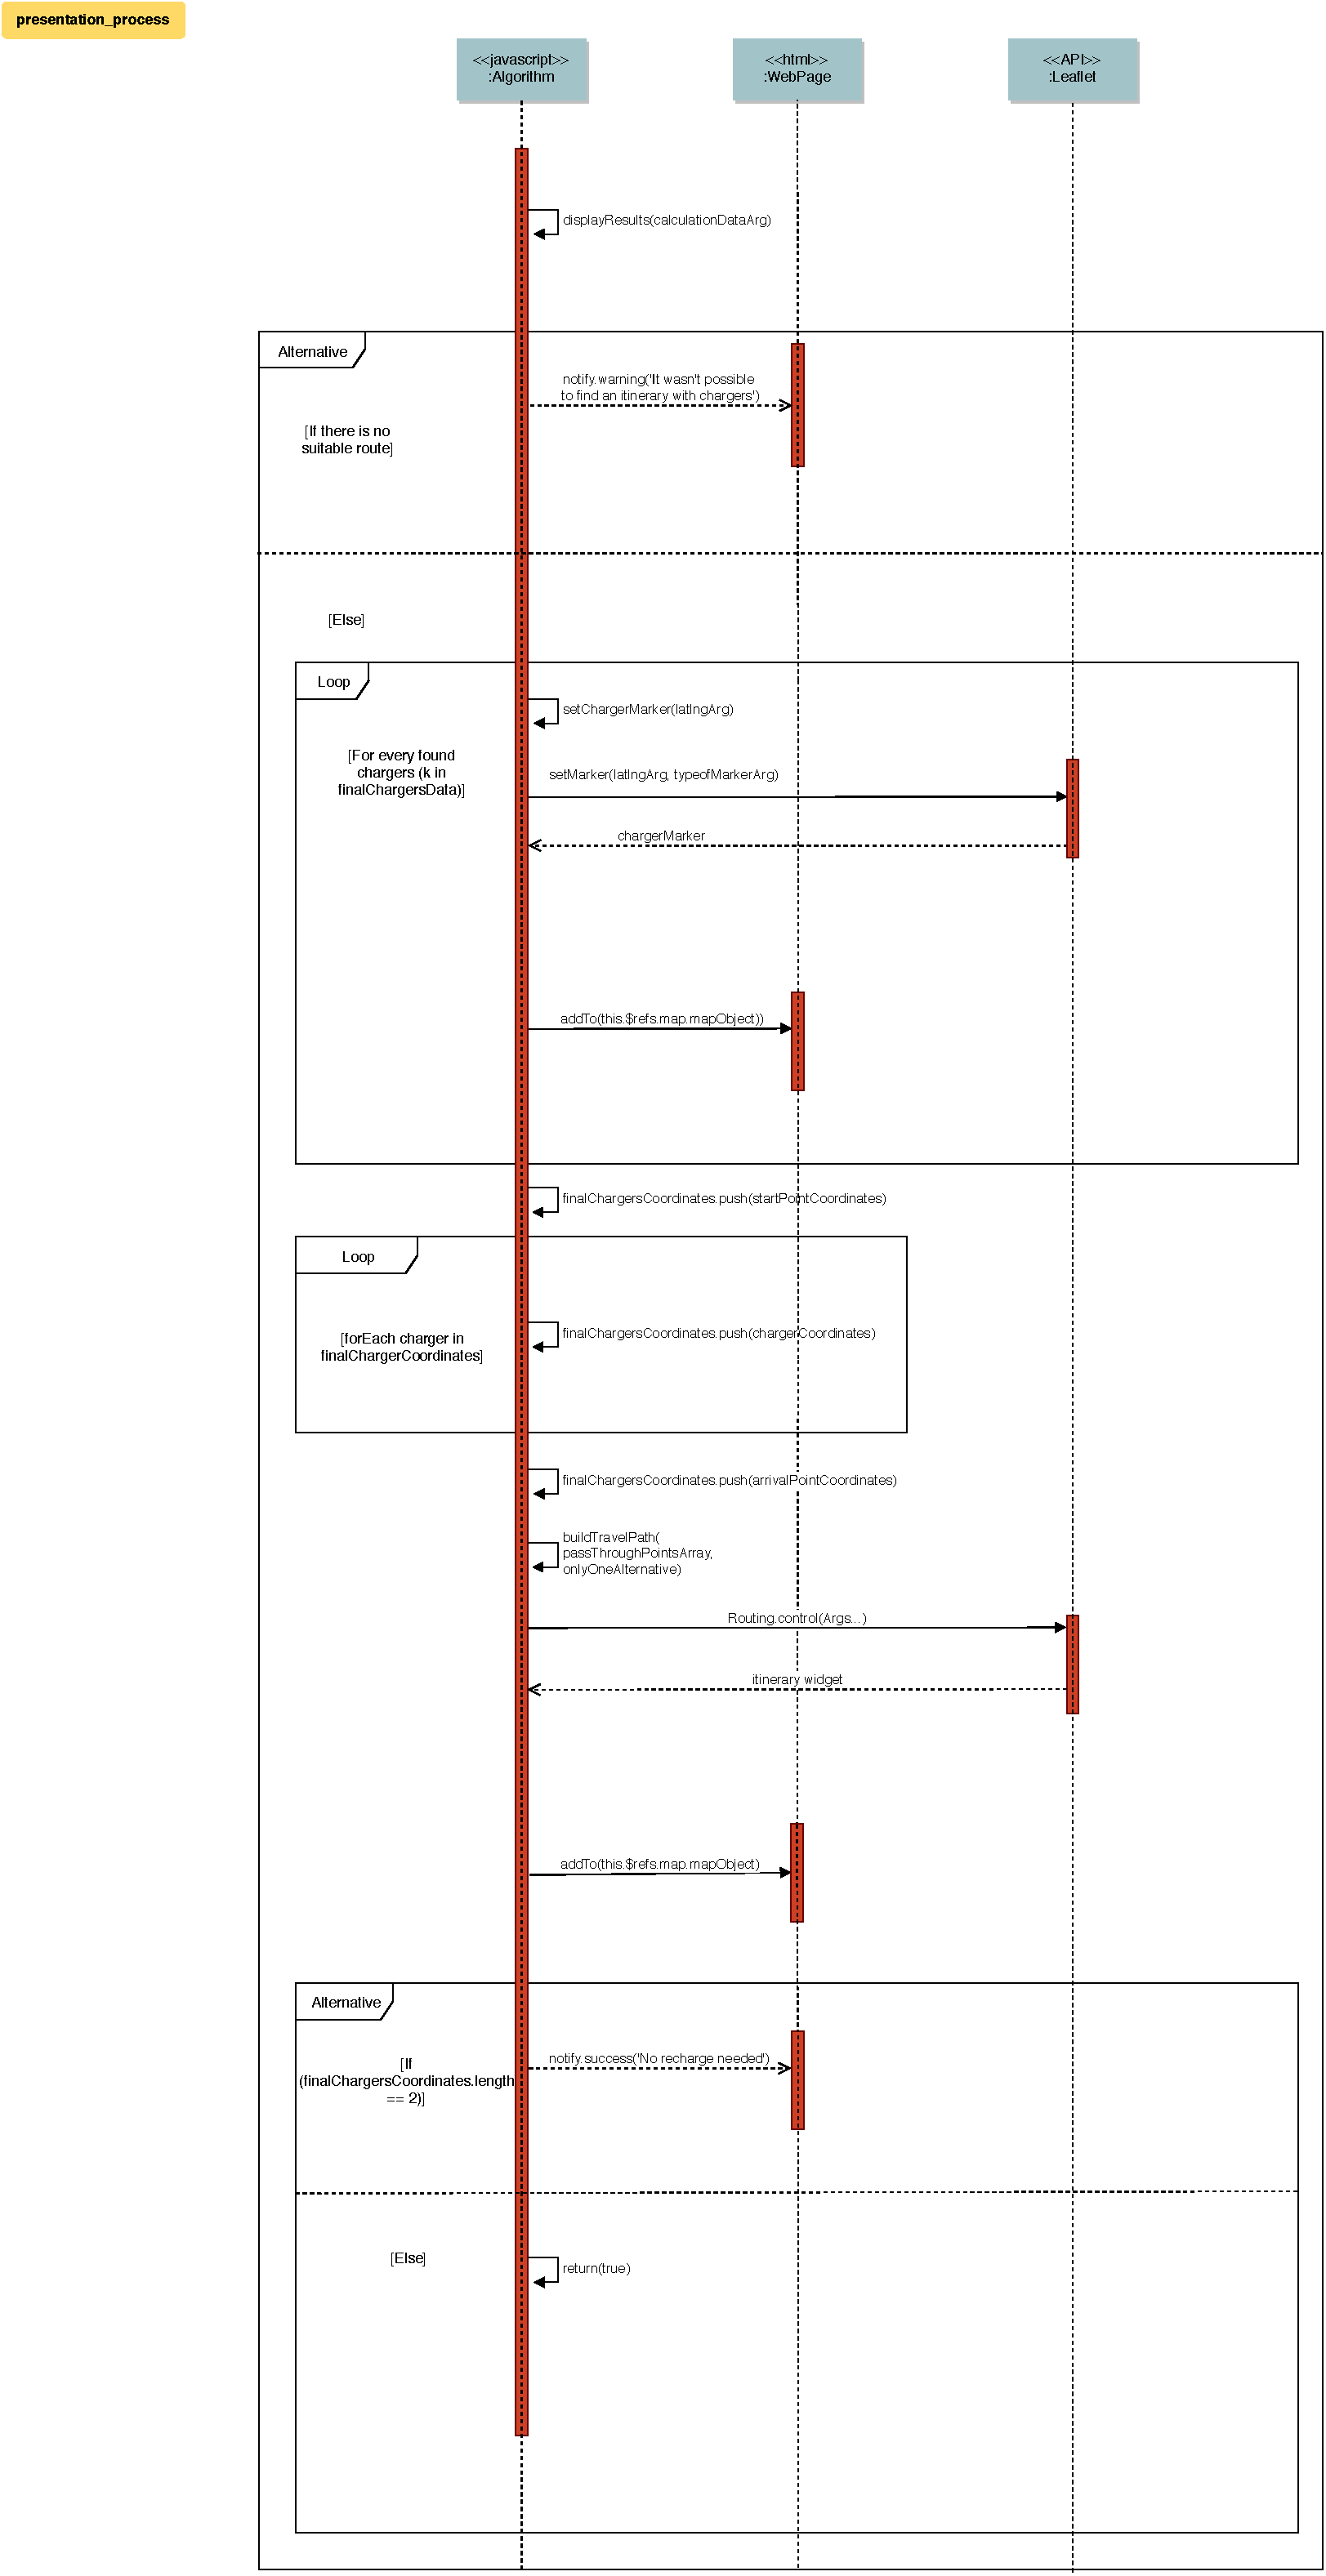
\includegraphics[scale=0.35]{Immagini/Presentation_SequenceDiagram.pdf}}
\caption{Template Deployment Diagram}
\end{figure}

\newpage

\section{Risultato dei Test} 
\hypertarget{section::\theHsection}
Il risultato dei test per questa iterazione è mostrato in figura. La suite composta da 3 test ha ricevuto esito positivo.

\begin{figure}[H]
\centering
{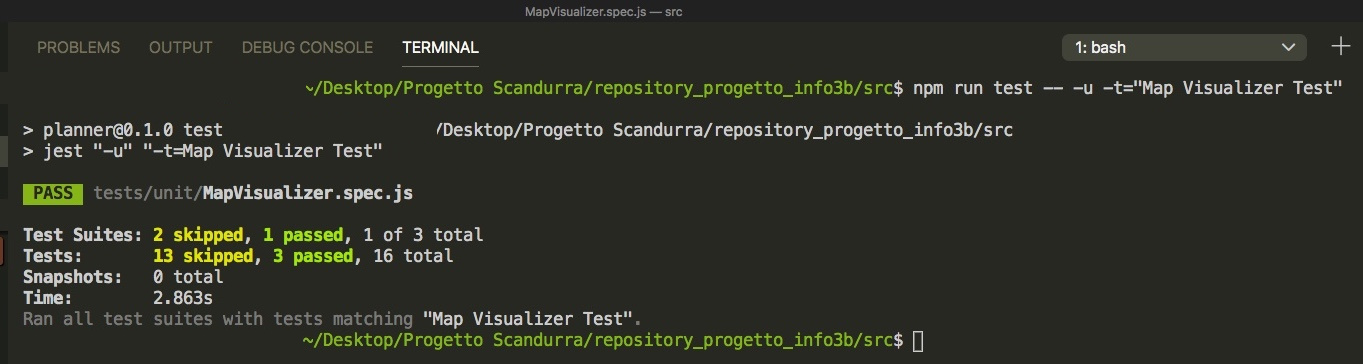
\includegraphics[scale=1]{Immagini/TestMapVisualizer.jpeg}}
\caption{Test iterazione 3}
\end{figure}

Presentiamo infine anche il risultato di tutte le suite di test per tutte le iterazioni eseguite contemporaneamente.

\begin{figure}[H]
\centering
{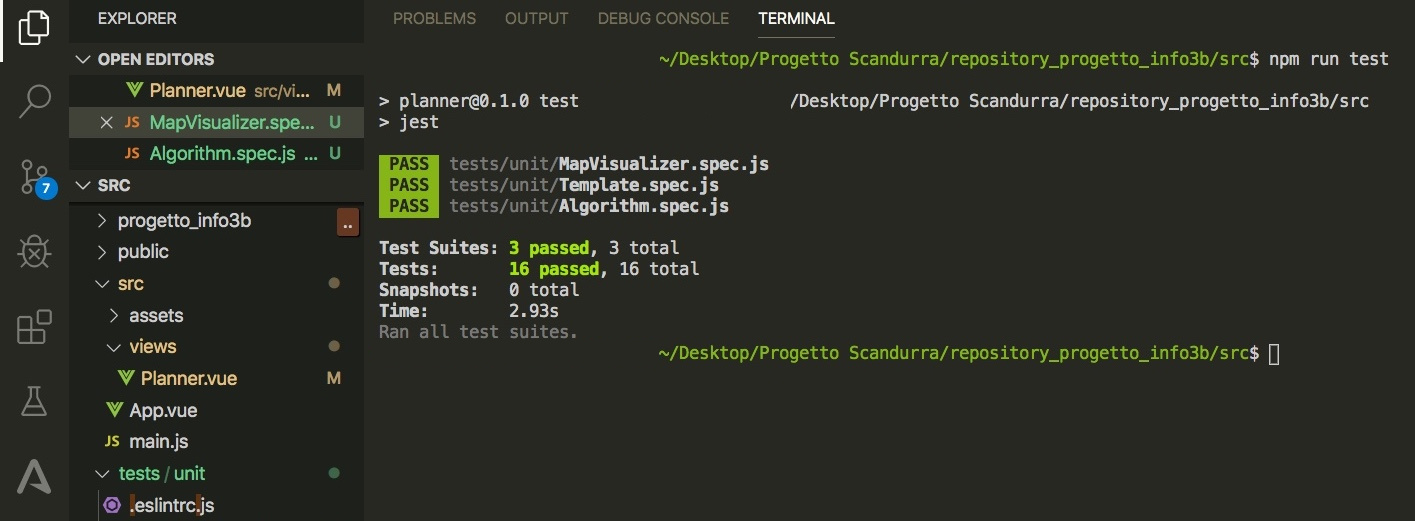
\includegraphics[scale=1]{Immagini/TestTotale.jpeg}}
\caption{Test completo}
\end{figure}


\chapter{Manuale Utente} \label{chap:Manuale utente} \hypertarget{chapter::\theHchapter}{}
\section{Installazione}
\hypertarget{section::\theHsection}
Per l'esecuzione del software sviluppato è necessario aprire l'applicazione in locale tramite le istruzioni di seguito riportate.

\lstinputlisting[language=Bash]{Codice/run_from_terminal.bash}

\begin{figure}[h]
\centering
{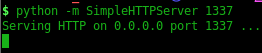
\includegraphics[scale=1]{Immagini/python_virtual_server.png}}
\caption{Virtual server in esecuzione}
\end{figure}

\newpage

Questa modalità di visualizzazione del sito presuppone che il sito sia già compilato per versione di produzione.

Se invece si volesse lanciare il sito dal codice sorgente, seguire le seguenti istruzioni.

\lstinputlisting[language=Bash]{Codice/run_from_terminal_versione_dev.bash}

\begin{figure}[h]
\centering
{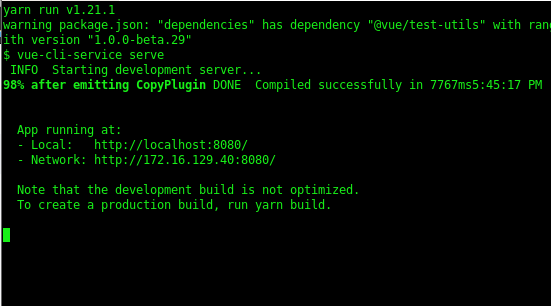
\includegraphics[scale=0.8]{Immagini/yarn_serve_localhost.png}}
\caption{"yarn serve" sito versione development in esecuzione}
\end{figure}

Il building si può fare con i seguenti commandi.

\lstinputlisting[language=Bash]{Codice/run_from_terminal_versione_build.bash}

\newpage

\begin{figure}[h]
\centering
{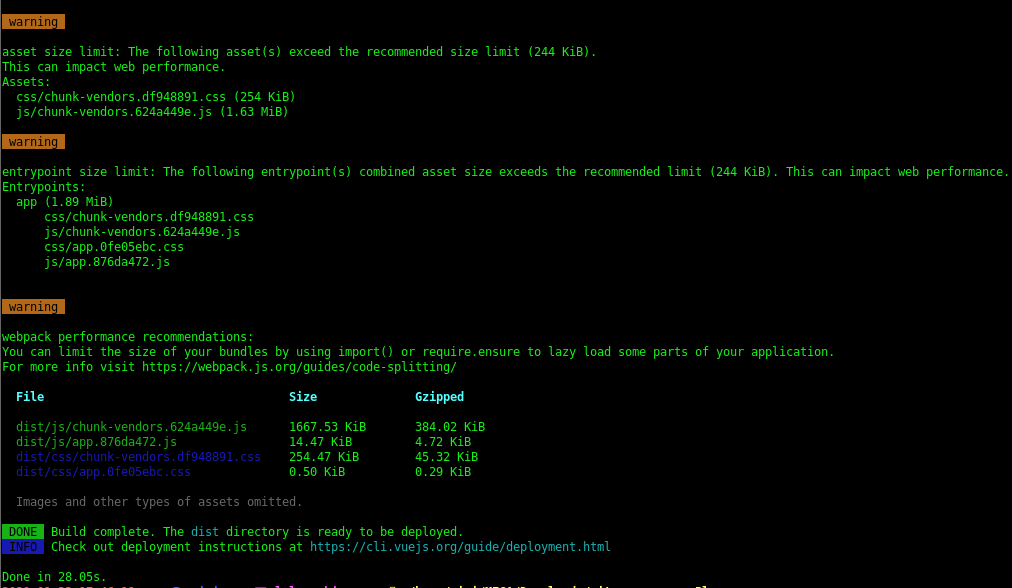
\includegraphics[scale=0.4]{Immagini/yarn_build_dist.png}}
\caption{"yarn build" compilazione del sito versione di produzione}
\end{figure}

\newpage

Una volta che le istruzioni sopra citate sono state eseguite verrà aperta una porta in locale nel proprio pc (ad.esempio http://localhost:8080/) con una schermata come riportato nella Figura 10.2. \autocite[\protect\label{Dayley2014}][]{Dayley2014}

Si procede aprendo un qualsiasi browser web e incollando l'indirizzo trovato nella barra di ricerca e premendo invio, il browser restituirà la Homepage della WebApp sviluppata.

\newpage

\section{Utilizzo}
\hypertarget{section::\theHsection}
In questa sezione verrà mostrato l'utilizzo dell'applicazione web sviluppata.
All'apertura della pagina web verrà mostrata una schermata contenente le caselle da riempire con i dati richiesti ed una mappa per la successiva visualizzazione.
Dopo l'inserimento dell'indirizzo sul proprio browser web verrà mostrato a schermo una pagina come nella Figura 10.4

La schermata è composta da 3 campi:
\begin{enumerate}
\item\textbf{Departure Address}: in questo campo deve essere inserita la città di partenza con l'eventuale indirizzo di partenza;
\item\textbf{Arrival Address}: in questo campo deve essere inserita la città di destinazione con l'eventuale indirizzo di destinazione;
\item\textbf{Car Autonomy}: in questo campo va inserita l'autonomia del proprio veicolo elettrico.
\end{enumerate}
\newpage
Il sistema è in grado di offrire dei suggerimenti riguardo l'inserimento delle destinazioni iniziali e finali e fare un check dei valori inseriti prima dell'invio al sistema.
In particolare nel campo autonomia non sono ammessi valori negativi ma soltanto valori compresi tra 1 e 1000 km.

\begin{figure}[h]
\centering
{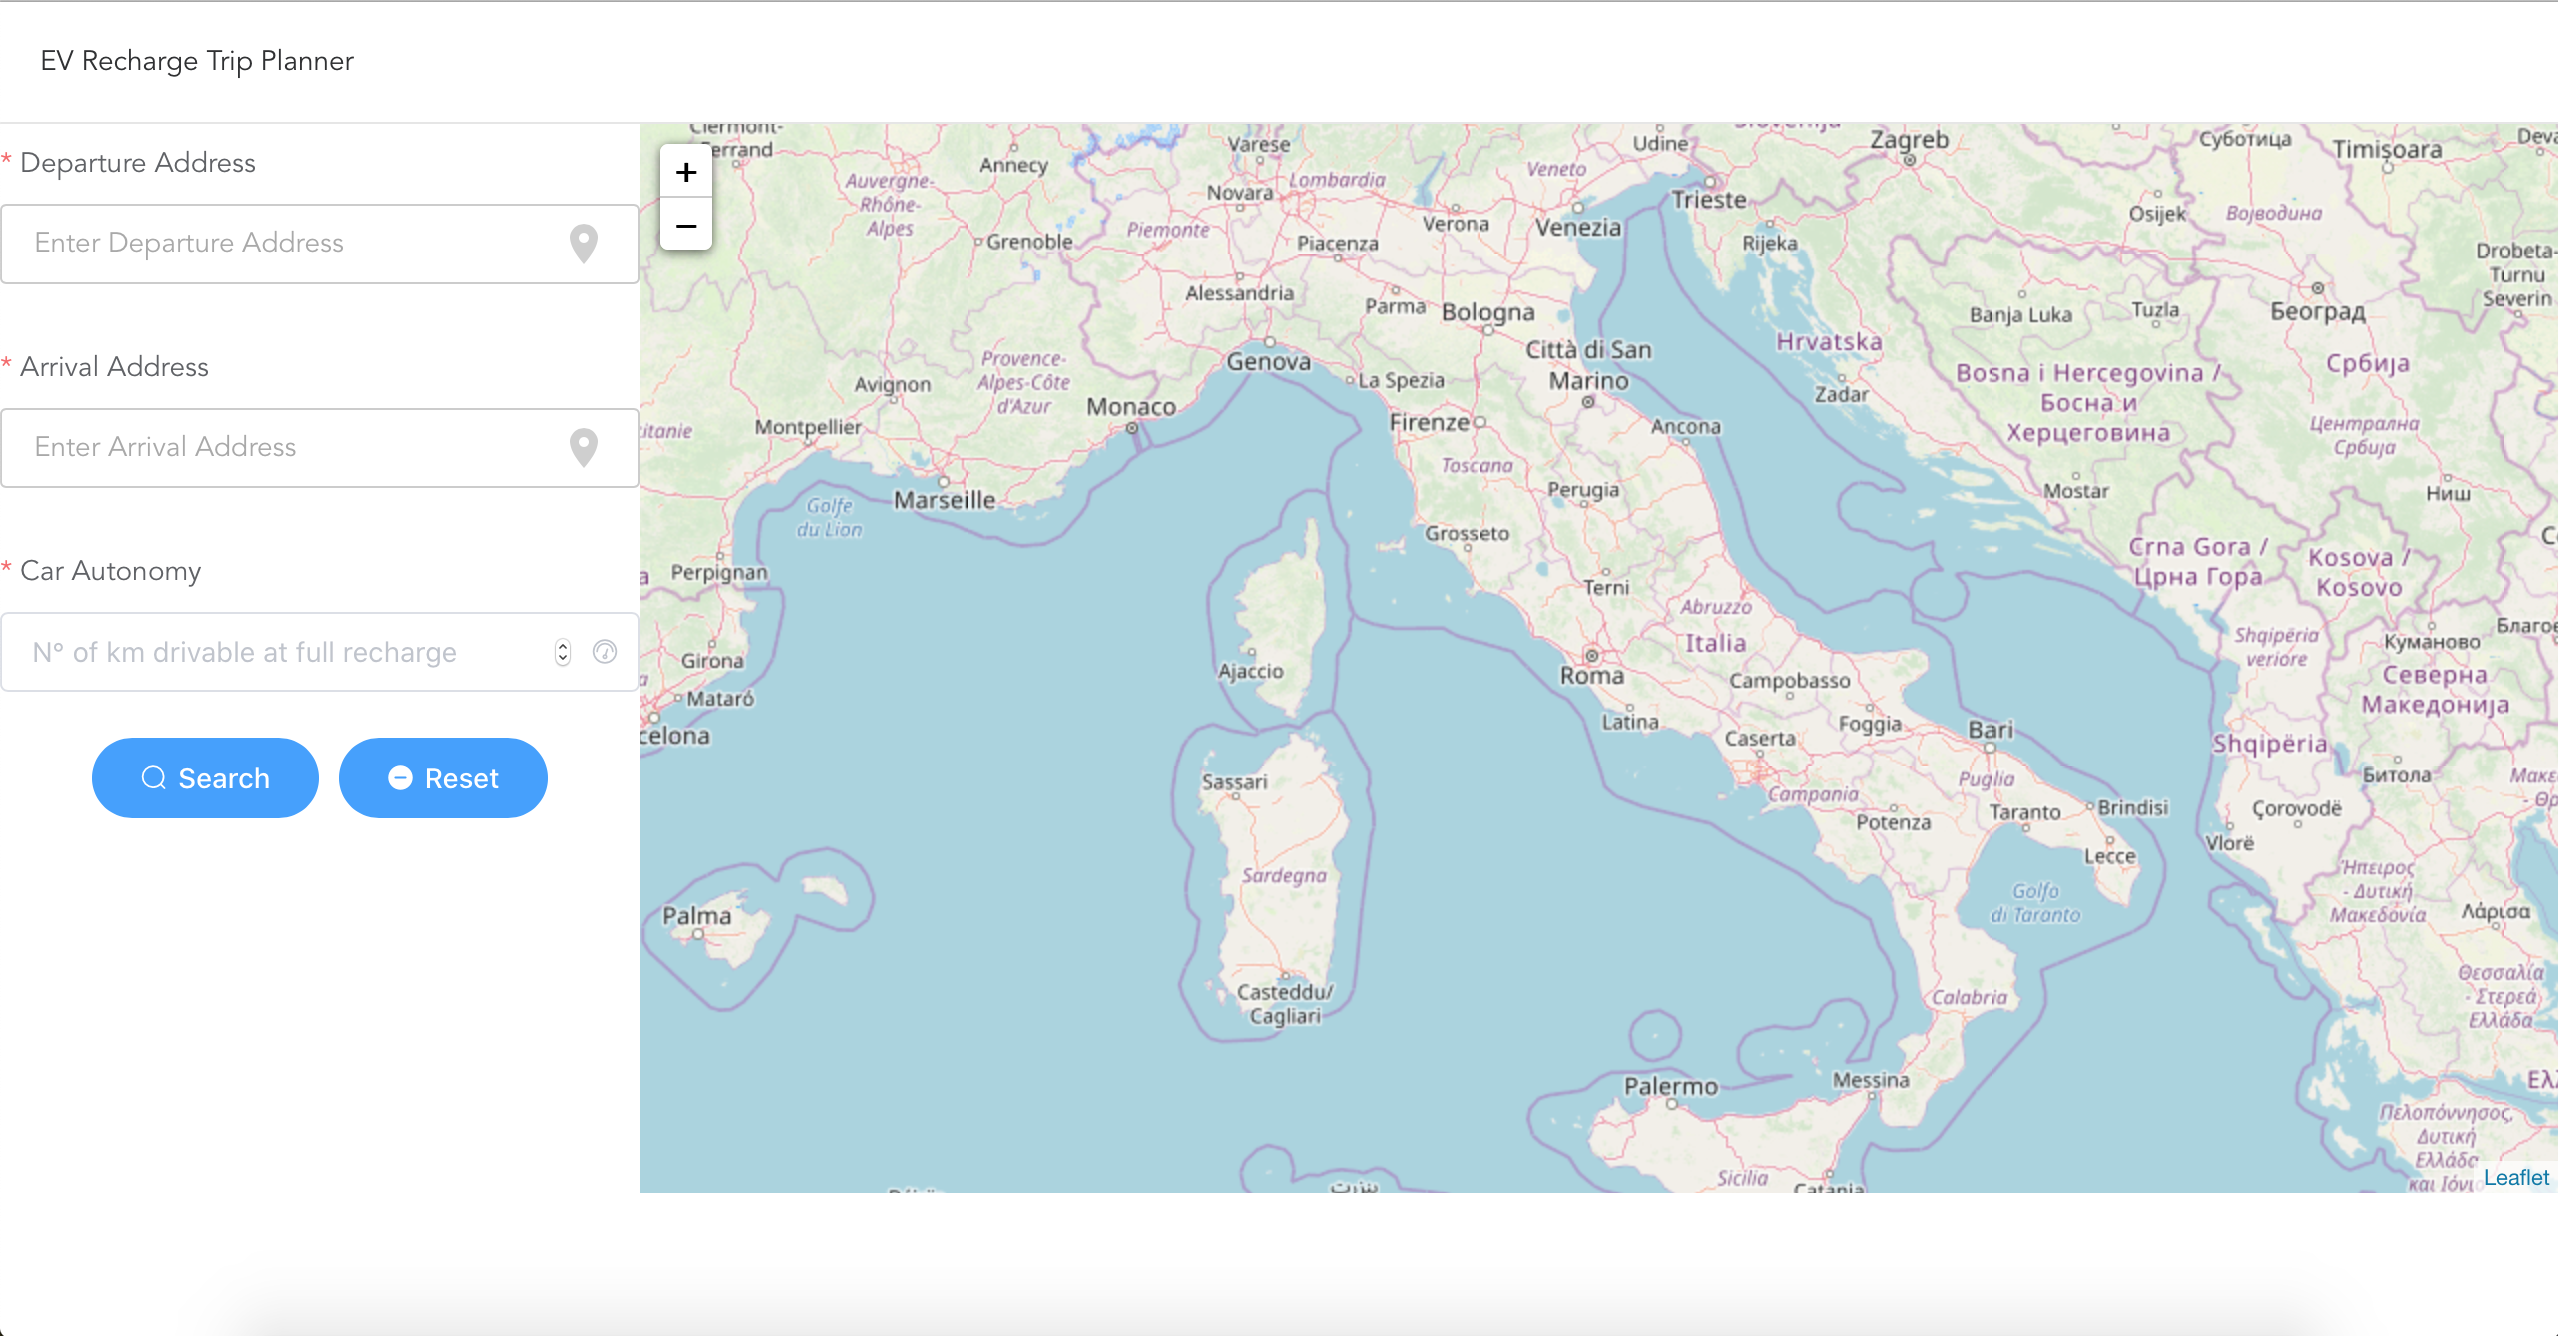
\includegraphics[scale=0.3]{Immagini/Schermata_Homepage.png}}
\caption{Schermata Homepage}
\end{figure}

Una volta inseriti nella schermata i dati 
richiesti, l'utente dovrà premere il pulsante Search come mostrato in Figura 10.5.

Il sistema risponderà con una schermata come in Figura 10.6 dove viene mostrato sulla mappa il punto iniziale e finale con il percorso da effettuare e le eventuali fermate.

\begin{figure}[h]
\centering
{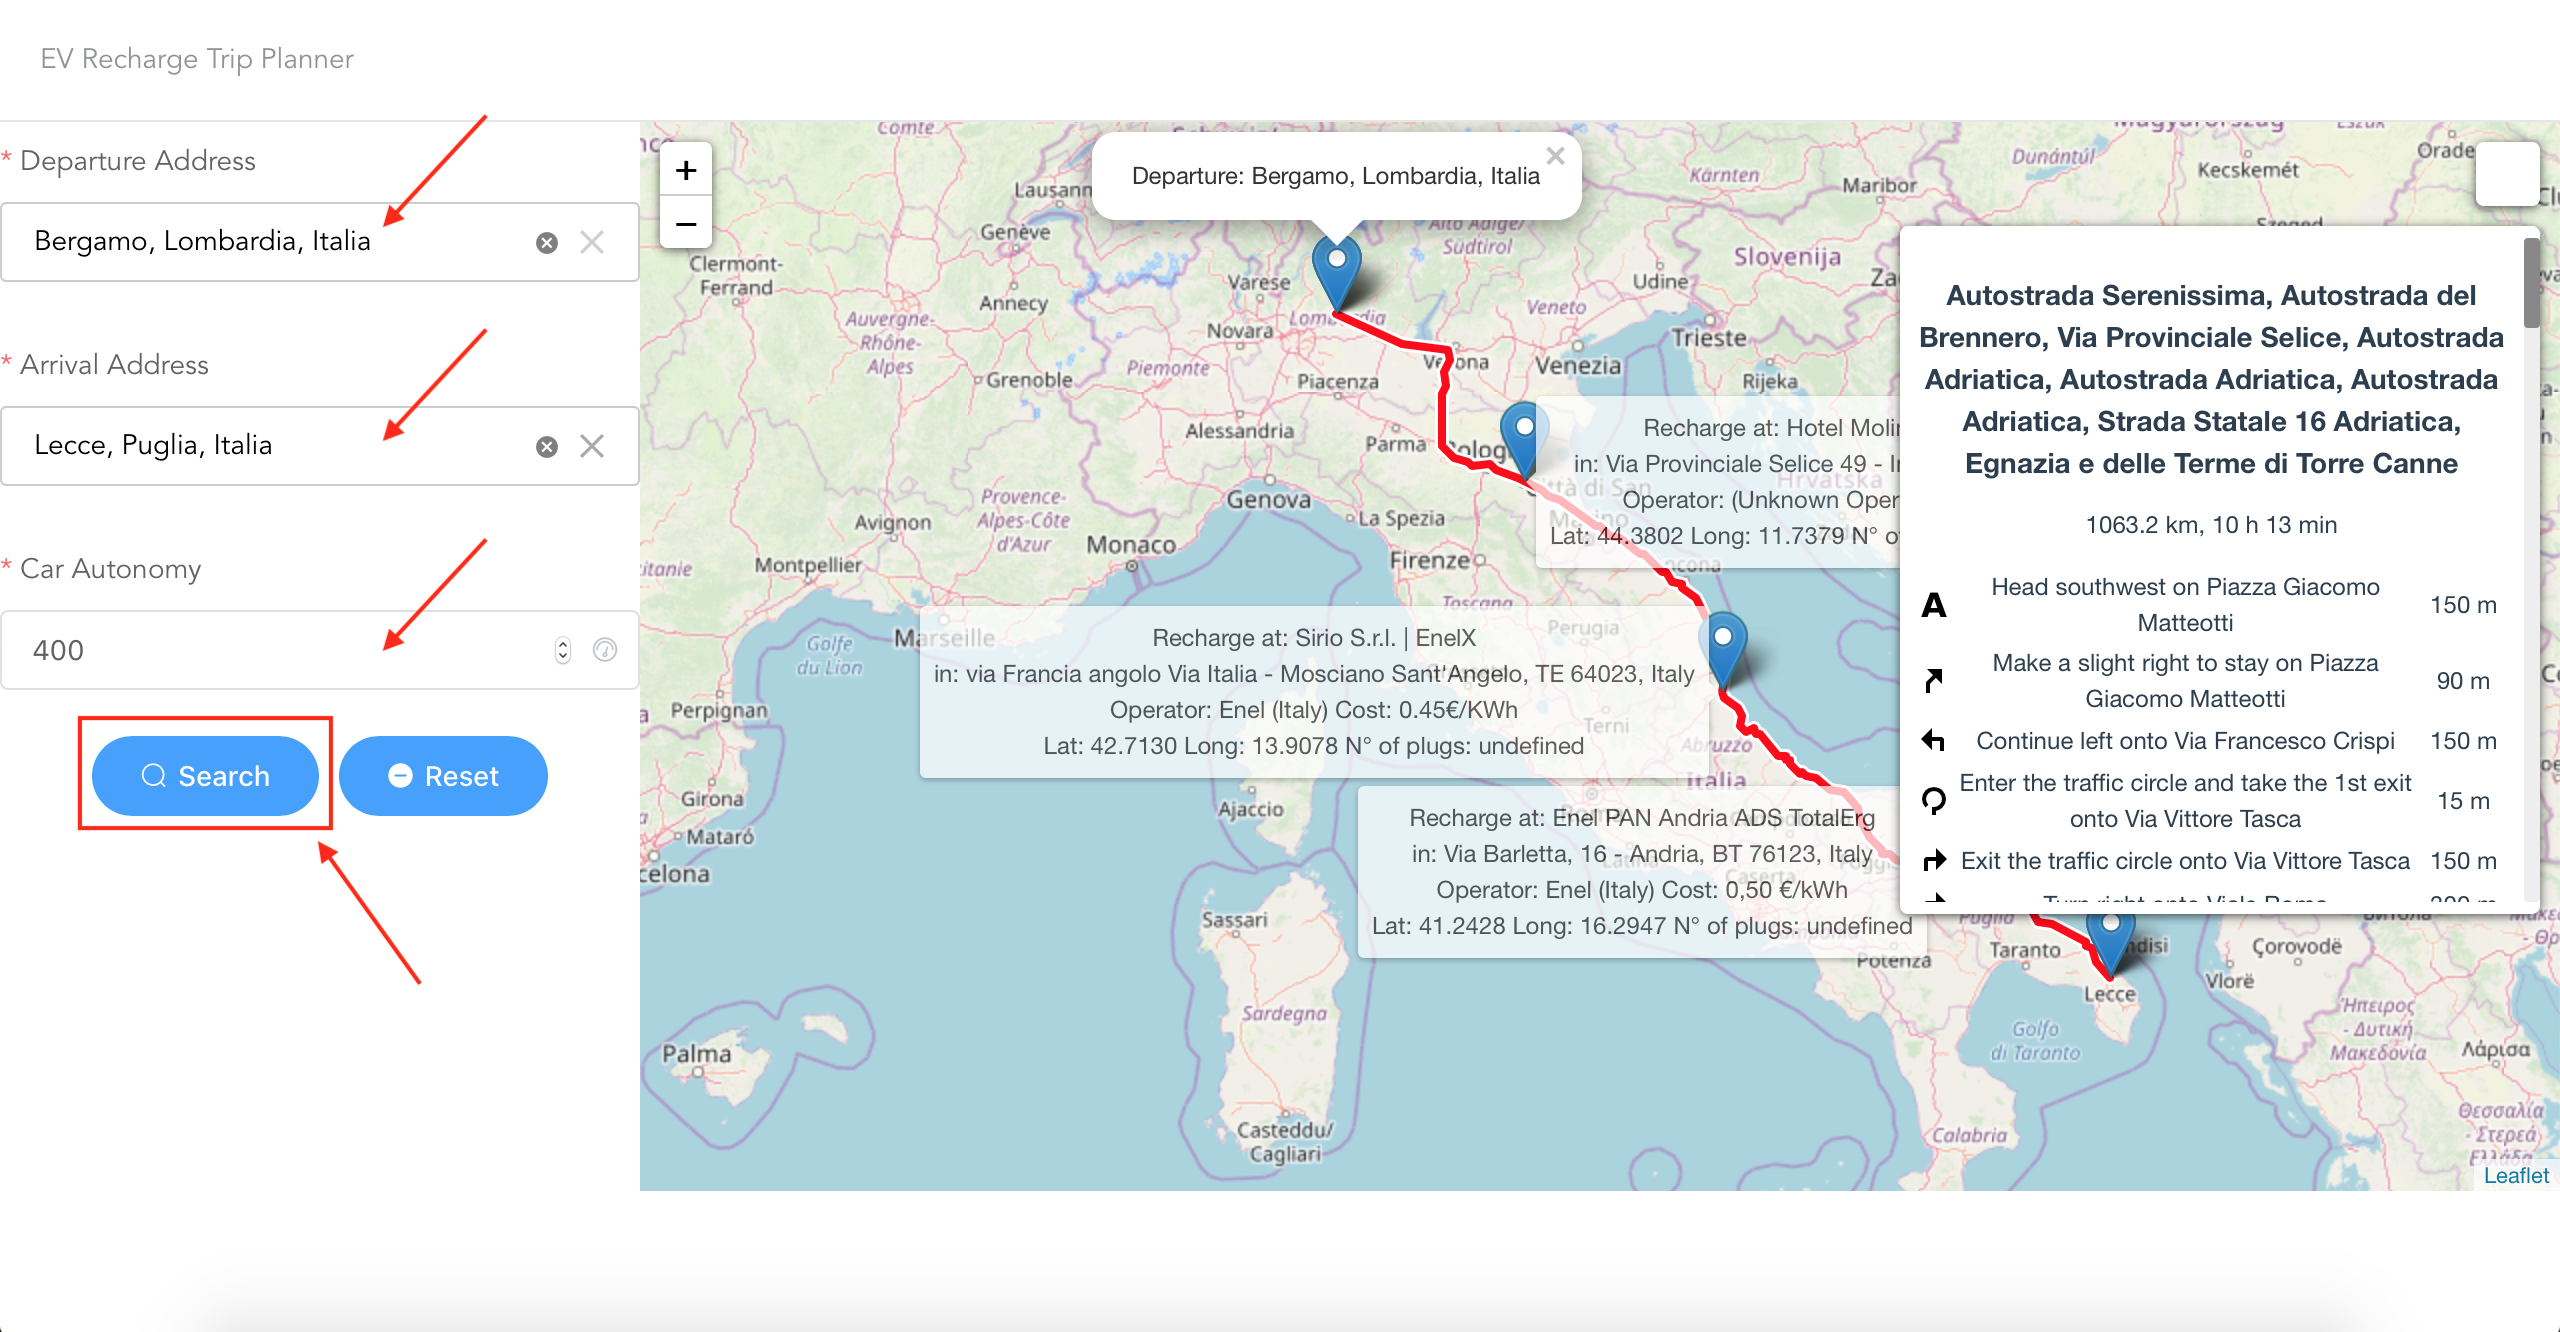
\includegraphics[scale=0.3]{Immagini/Schermata_esempio_planner_2.png}}
\caption{Schermata Esempio Planner}
\end{figure}
\newpage
In particolare vengono mostrate sulla mappa le fermate da effettuare con il nome della colonnina di ricarica, la via in cui essa è situata, l'operatore erogatore del servizio, il costo della colonnina e il numero di prese di corrente disponibili.

Inoltre compare una finestra a tendina interattiva dove sono mostrate le indicazioni dettagliate da seguire per raggiungere il posto desiderato.
La tendina è scorribile in lunghezza e posizionando la freccia su una specifica indicazione è possibile vedere sulla mappa tramite un cerchio blu dove corrisponde l'indicazione sulla mappa.

\begin{figure}[h]
\centering
{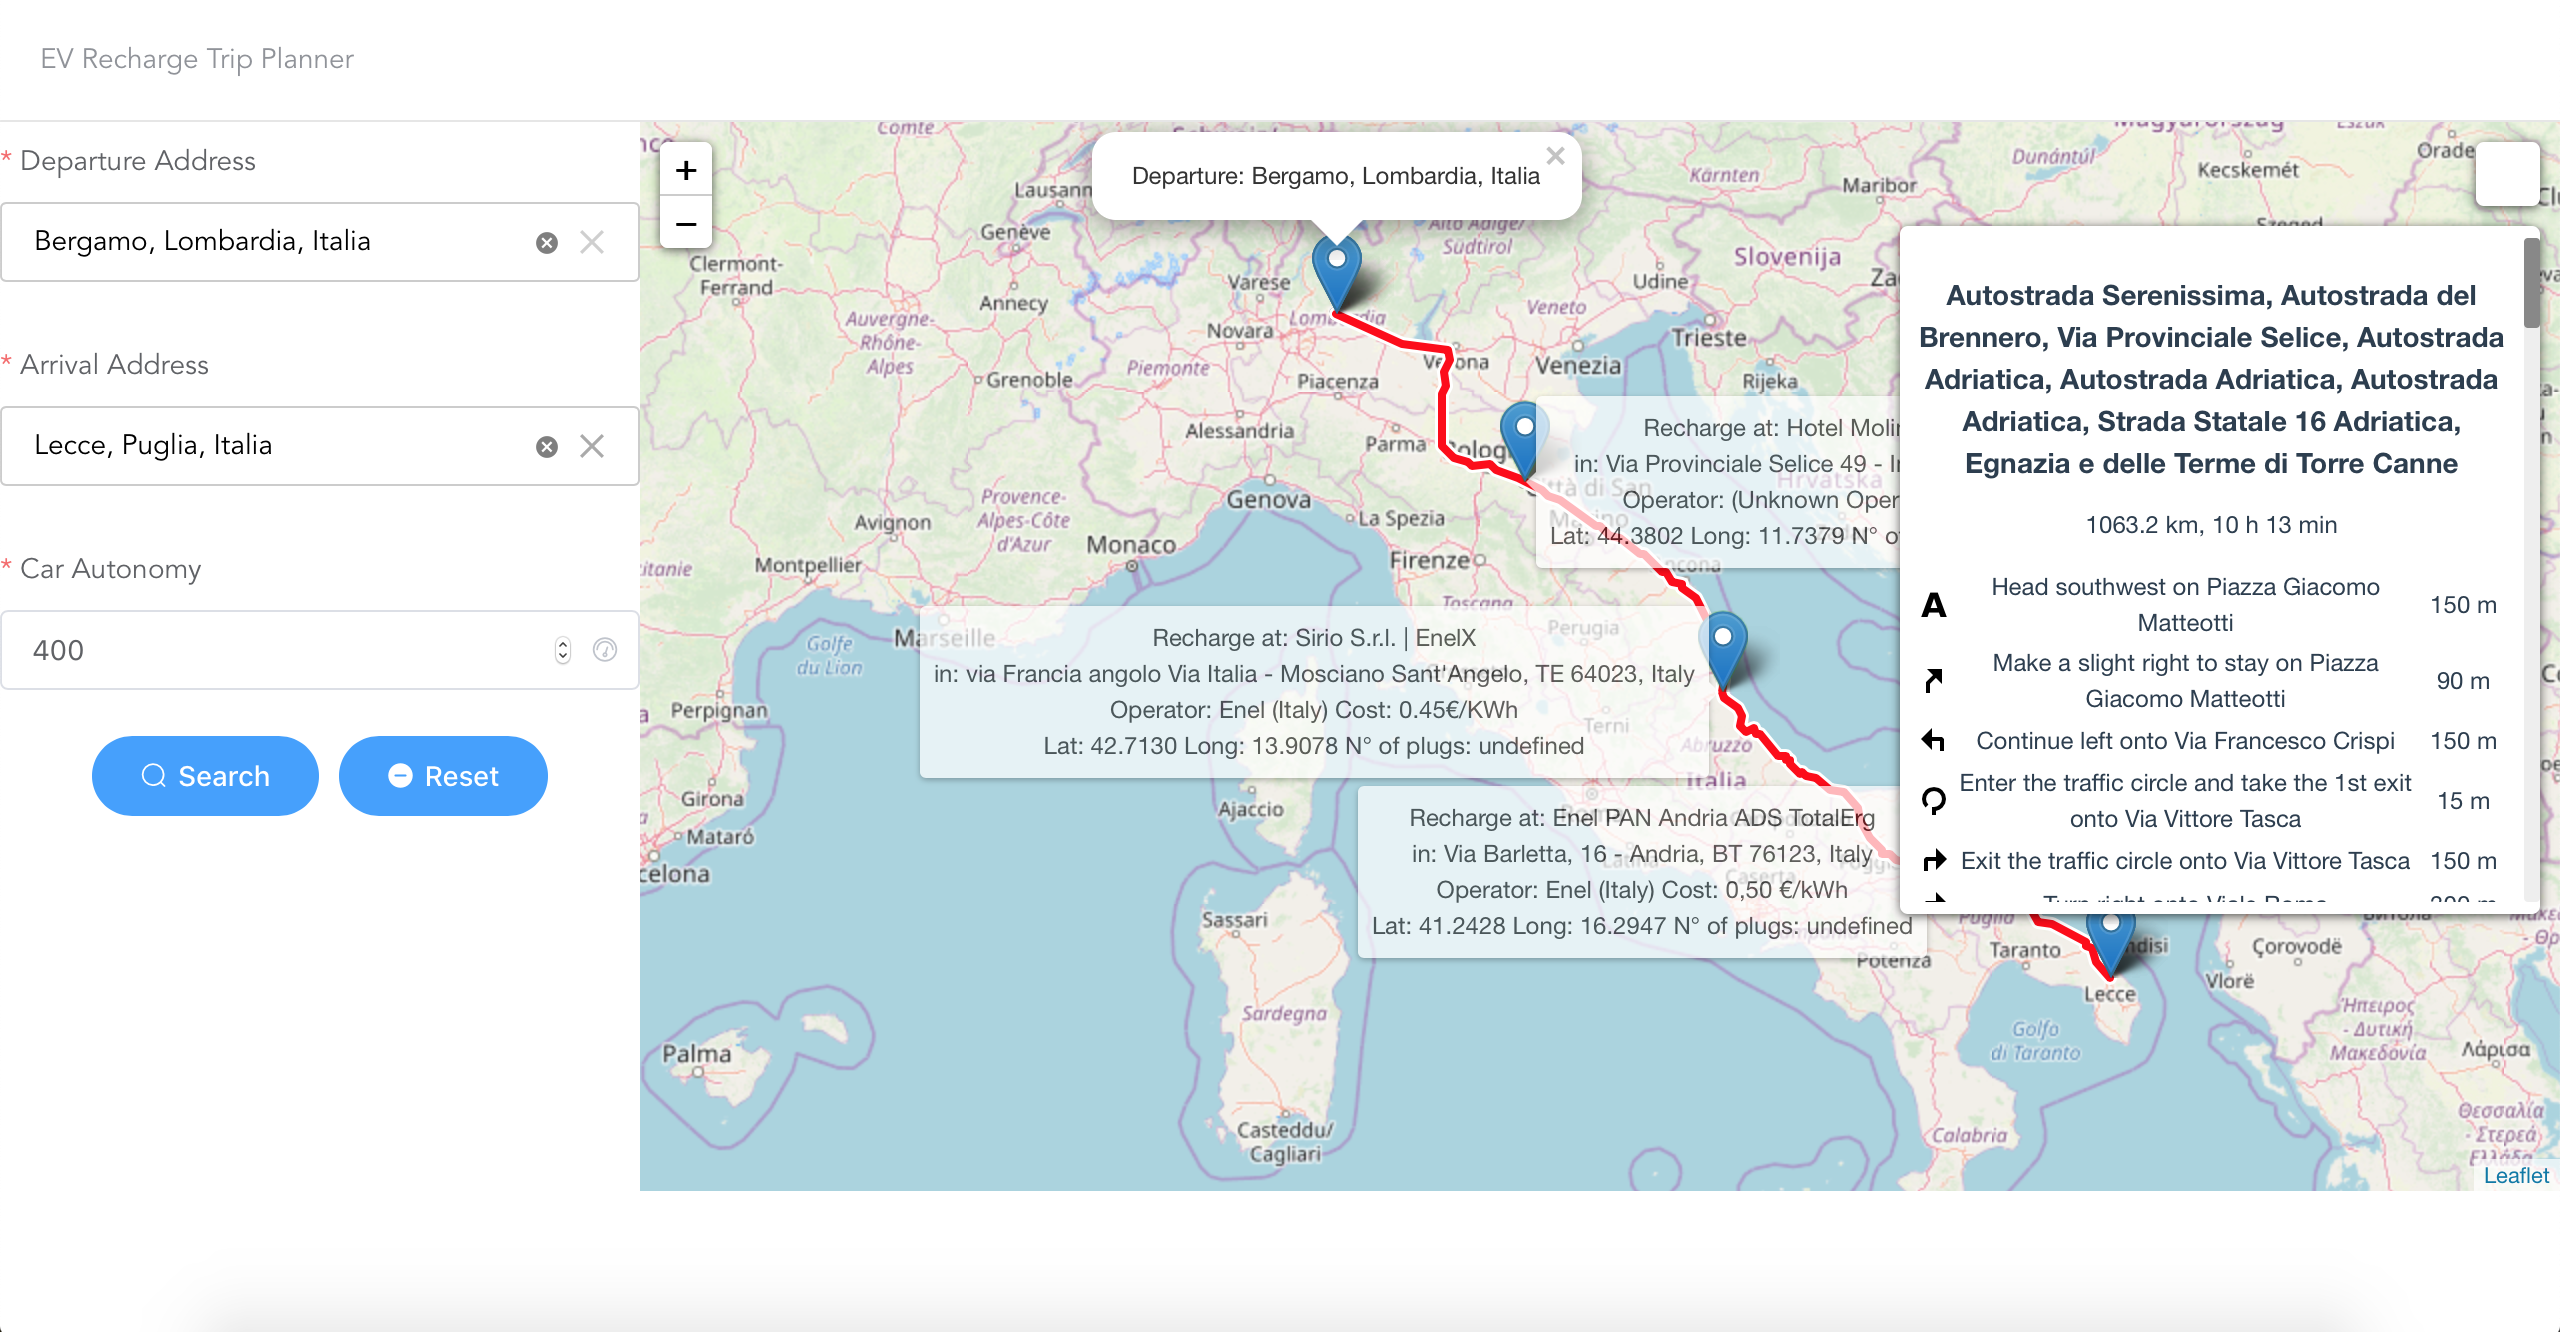
\includegraphics[scale=0.3]{Immagini/Schermata_esempio_planner.png}}
\caption{Schermata Esempio Planner 2}
\end{figure}

Una volta che l'utente ha visualizzato un determinato percorso esso potrà cancellare quello appena cercato ed effettuarne uno nuovo tramite il pulsante Reset come mostrato in Figura 10.7, la schermata che si presenterà è identica alla Homepage del programma.

\begin{figure}[h]
\centering
{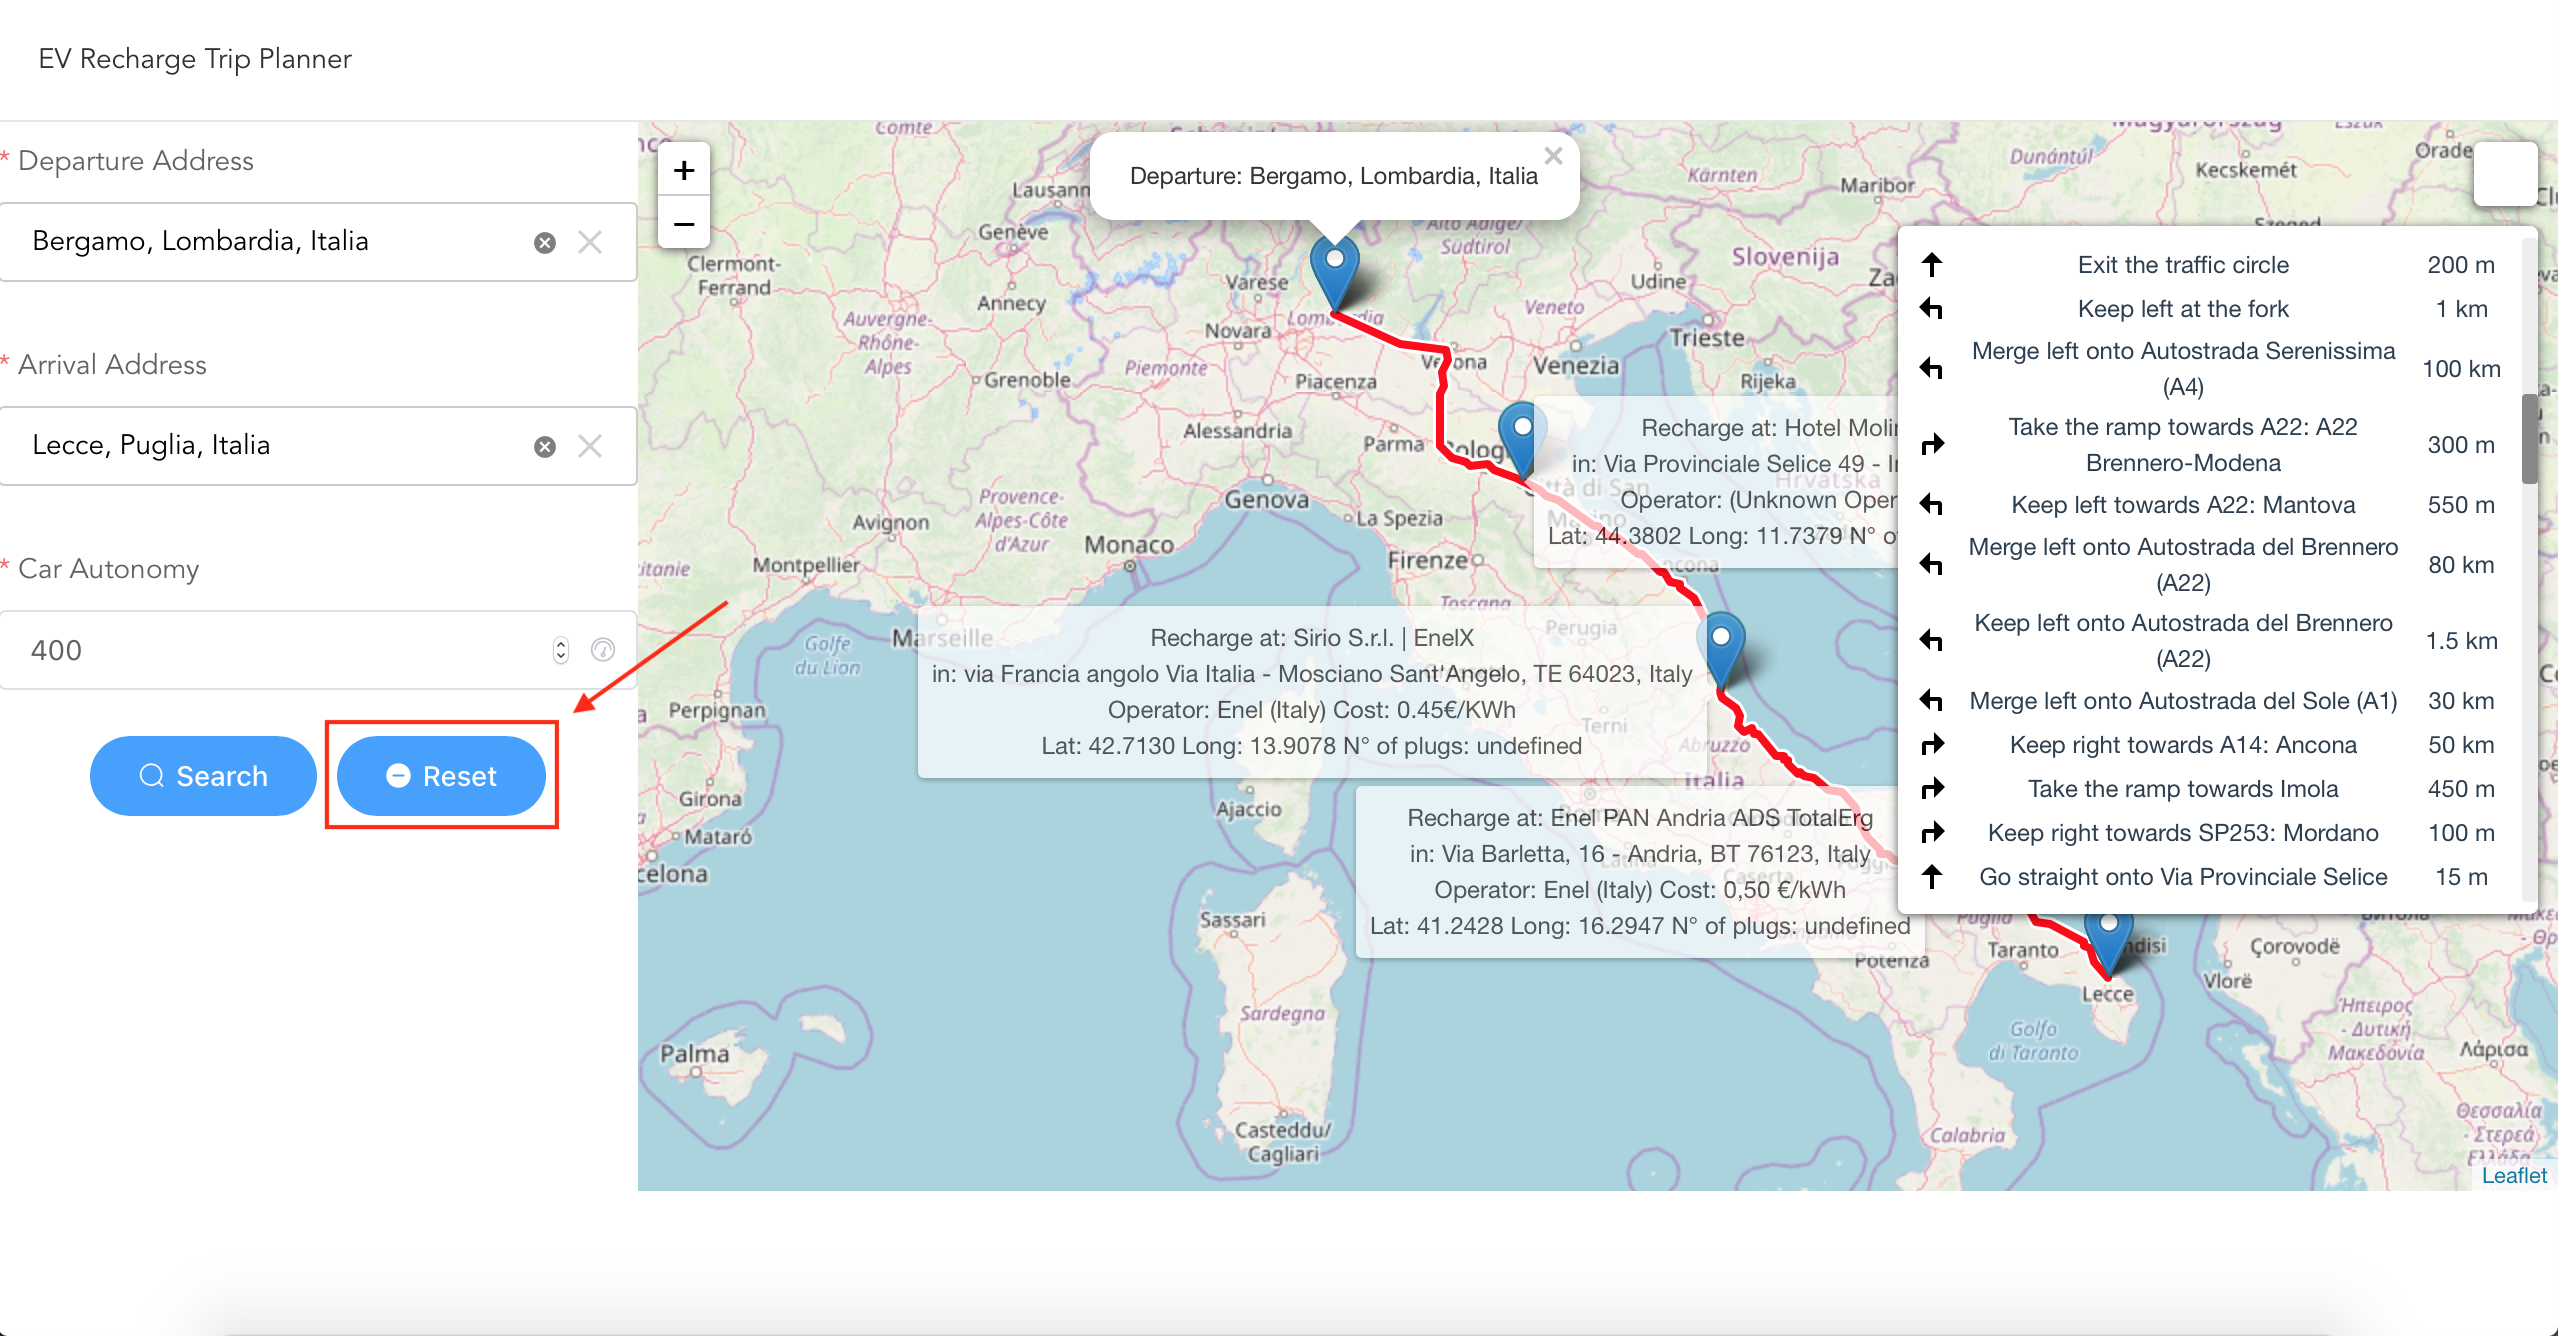
\includegraphics[scale=0.3]{Immagini/Schermata_esempio_planner_Reset.png}}
\caption{Schermata Esempio Planner 3}
\end{figure}







\chapter{Toolchain} \label{chap:Toolchain} \hypertarget{chapter::\theHchapter}{}
\section{Tools}
\hypertarget{section::\theHsection}
Per realizzare il nostro progetto ci siamo avvalsi dei seguenti tool:
\begin{enumerate}
\item termux: terminale per mobile
\item python: linguaggio di programmazione usato per "runnare" il server virtuale
\item http-server: server virtuale per runnare siti web
\item Visual Studio: IDE di sviluppo general purpose
\item SublimeText: text editor per sviluppo general purpose
\item pkg: package manager per terminale mobile
\item pip: python package manager
\item Mozilla Firefox: Web Browser
\item Safari: Web Browser
\item Chromium : Web Browser
\item Konsole: terminale per ambiente GNU/Linux
\item tmux: multiplexer di finestre di terminale
\item gigle: software per GUI git, gestione branch e versioning
\item inspector: web browser debugging tool
\item evince: pdf document viewer
\item inkscape: editore di immagini e documenti raster
\item Git Cola: GUI software per la gestione dei branch e versioning git
\item Mocha: libreria per VueJS testing
\item Synaptic Package Manager: package manager per sistemi GNU/Linux
\item Jest: libreria per VueJs testing
\item ESlint: analisi statica del codice
\item Mega: servizio di archiviazione e backup online
\item Brackets: IDE per sviluppo HTML e CSS
\item WireShark: software per catturare ed analizzare pacchetti scambiati durante le interrogazioni alle API
\item Github: sito di hosting di repository
\item WebPack: module bundler e minimizer per applicazioni JavaScript
\item SourceTree: client di gestione versioning con GUI git
\item Eclipse: IDE per la programmazione in Java
\item WebStorm: IDE per programma in VueJS Framework di Javascript
\item NodeJS: gestore di moduli e librerie per sviluppo di siti web
\item Yarn: package manager
\item Bitbucket: servizio web per la gestione di repository git
\item Overleaf: servizio web per la creazione e archiviazione di documenti \LaTeX. Consente inoltre la collaborazione di più utenti sullo stesso documento in tempo reale
\item Draw.io: servizio Web per la creazione di grafici fra cui anche i diagrammi UML
\item Telegram: app di messaggistica
\end{enumerate}

\section{Librerie}
\hypertarget{section::\theHsection}
Per la realizzazione del nostro progetto ci siamo avvalsi delle seguenti librerie:

\begin{enumerate}
\item Leaflet
\item Vue2 leaflet
\item vue places
\item leaflet routing machine
\item leaflet control geocoder
\item axios
\end{enumerate}

%\cleardoublepage

\bookmarksetup{startatroot}
\addtocontents{toc}{\bigskip}

\backmatter
\printbibliography[title=Bibliografia, heading=bibintoc] \label{Bibliografia}
\newpage

{\chapter*{}
\hypertarget{Coverback}{}
\label{Copertina_dietro} \thispagestyle{empty}}
\end{document}